\documentclass{beamer}  % presen 12pt
\mode<presentation>
%\usepackage{hyperref}
\usetheme{Madrid}
\usepackage{beamerthemesplit}
\usepackage[export]{adjustbox}
\usepackage{color}
\usepackage{tikz}
%

\input{../../Lab/stylefiles/rules/MyPackages}
% Font
\input{../../Lab/stylefiles/rules/MyBold}
\input{../../Lab/stylefiles/rules/MyCal}
\input{../../Lab/stylefiles/rules/MyScr}
\input{../../Lab/stylefiles/rules/MyBB}
\input{../../Lab/stylefiles/rules/MyTilde}
\input{../../Lab/stylefiles/rules/MyBar}
\input{../../Lab/stylefiles/rules/MyHat}
\input{../../Lab/stylefiles/rules/MyRoman}
% Environment
\input{../../Lab/stylefiles/rules/MyOperations}
\input{../../Lab/stylefiles/rules/MyNewEnvironment}
% References
\input{../../Lab/stylefiles/rules/MyJournals}
\bibliographystyle{IEEEtran}
\usepackage{graphicx}
\usepackage{lscape}
\usepackage{beamerthemesplit}
\setbeamertemplate{navigation symbols}{}
\setbeamertemplate{footline}[frame number]
\usetheme{Luebeck}
\renewcommand{\figurename}{図}
\renewcommand{\tablename}{表}
%\usepackage{xeCJK}
%\setCJKmainfont{MS Gothic}
%

\input{../../Lab/stylefiles/rules/MyPackages}
% Font
\input{../../Lab/stylefiles/rules/MyBold}
\input{../../Lab/stylefiles/rules/MyCal}
\input{../../Lab/stylefiles/rules/MyScr}
\input{../../Lab/stylefiles/rules/MyBB}
\input{../../Lab/stylefiles/rules/MyTilde}
\input{../../Lab/stylefiles/rules/MyBar}
\input{../../Lab/stylefiles/rules/MyHat}
\input{../../Lab/stylefiles/rules/MyRoman}
% Environment
\input{../../Lab/stylefiles/rules/MyOperations}
\input{../../Lab/stylefiles/rules/MyNewEnvironment}
% References
\input{../../Lab/stylefiles/rules/MyJournals}
\bibliographystyle{IEEEtran}
\usepackage{graphicx}
\usepackage{lscape}
\usepackage{beamerthemesplit}
\setbeamertemplate{navigation symbols}{}
\setbeamertemplate{footline}[frame number]
\usetheme{Luebeck}
\renewcommand{\figurename}{図}
\renewcommand{\tablename}{表}

\newcommand\blfootnote[1]{%
  \begingroup
  \renewcommand\thefootnote{}\footnote{#1}%
  \addtocounter{footnote}{-1}%
  \endgroup
}

% limits underneath
\DeclareMathOperator*{\argminA}{arg\,min} % Jan Hlavacek
\DeclareMathOperator*{\argminB}{argmin}   % Jan Hlavacek
\DeclareMathOperator*{\argminC}{\arg\min}   % rbp

\newcommand{\argminD}{\arg\!\min} % AlfC

\newcommand{\argminE}{\mathop{\mathrm{argmin}}}          % ASdeL
\newcommand{\argminF}{\mathop{\mathrm{argmin}}\limits}   % ASdeL

% limits on side
\DeclareMathOperator{\argminG}{arg\,min} % Jan Hlavacek
\DeclareMathOperator{\argminH}{argmin}   % Jan Hlavacek
\newcommand{\argminI}{\mathop{\mathrm{argmin}}\nolimits} % ASdeL

\newcommand{\cs}[1]{\texttt{\symbol{`\\}#1}}




\title[Deterministic Interleaver Design for Turbo Codes]{Deterministic Interleaver Design for Turbo Codes}
\author[Bohulu]{ Bohulu Kwame Ackah, 1631133 }
\institute[UEC]{Information Transmission Labroratory}
\date[Week 3]{\today}
\begin{document}
\frame{\titlepage}

\addtobeamertemplate{navigation symbols}{}{%
    \usebeamerfont{footline}%
    \usebeamercolor[fg]{footline}%
    \hspace{1em}%
    \insertframenumber/\inserttotalframenumber
}

\begin{frame}

	\frametitle{1. Turbo Codes : Brief Introduction}
	\begin{itemize}
\setlength\itemsep{2em}
	\item AWGN channel capacity approacing code

\item Parallel concatenation of 2 convolutional codes via an interleaver

	\item Good performance depends on interleaver
	\end{itemize}
	% \footnote{RSC : Recursive Systematic Convolutional}
\end{frame}

%slide 2
\begin{frame}
\frametitle{2. Interleavers}


\begin{itemize}
\setlength\itemsep{2em} 

\item Divided into 2 groups
\begin{itemize}
\setlength\itemsep{1em}
\item Random Interleavers
\begin{itemize}
\item Advantage: Good performance for large frame sizes

\item Disadvantage: storage of interleaver tables required.
\end{itemize}
\item Deterministic Interleavers
\begin{itemize}
\item Advantage : Interleaving done via algorithm

\item Disadvantage: For large frame sizes, interleaver better than random not yet found.

\item Design is very challenging


\end{itemize}
\end{itemize}
%\item PPI used as 4G LTE standard
\end{itemize}
\blfootnote {[5] Jing Sun, Oscar Y. Takeshita ''Interleavers for Turbo Codes Using 
Permutation Polynomials over Integer Rings'', IEEE Trans. Inform. Theory, vol. 51, 
pp. 101 - 119  Jan. 2005.}
\end{frame}


\begin{frame}
\frametitle{3. Purpose of Research}
\begin{itemize}
\setlength\itemsep{2em}

\item Main Goal of Research 

\begin{itemize}
\item Deterministic interleaver that outperforms random interleaver for large frame sizes
\end{itemize}

\item Current Step

\begin{itemize}
\item Deterministic interleaver that outperforms linear interleaver for large frame sizes

\item multi-shift interleaver is proposed
\end{itemize}

\item Why Linear Interleaver?
\begin{itemize}
\item Better than random interleaver for short frame sizes.

\item Easy to design
\end{itemize}

\end{itemize}
\end{frame}

\begin{frame}
\frametitle{4. Turbo Encoder}

\begin{figure}
\centering
		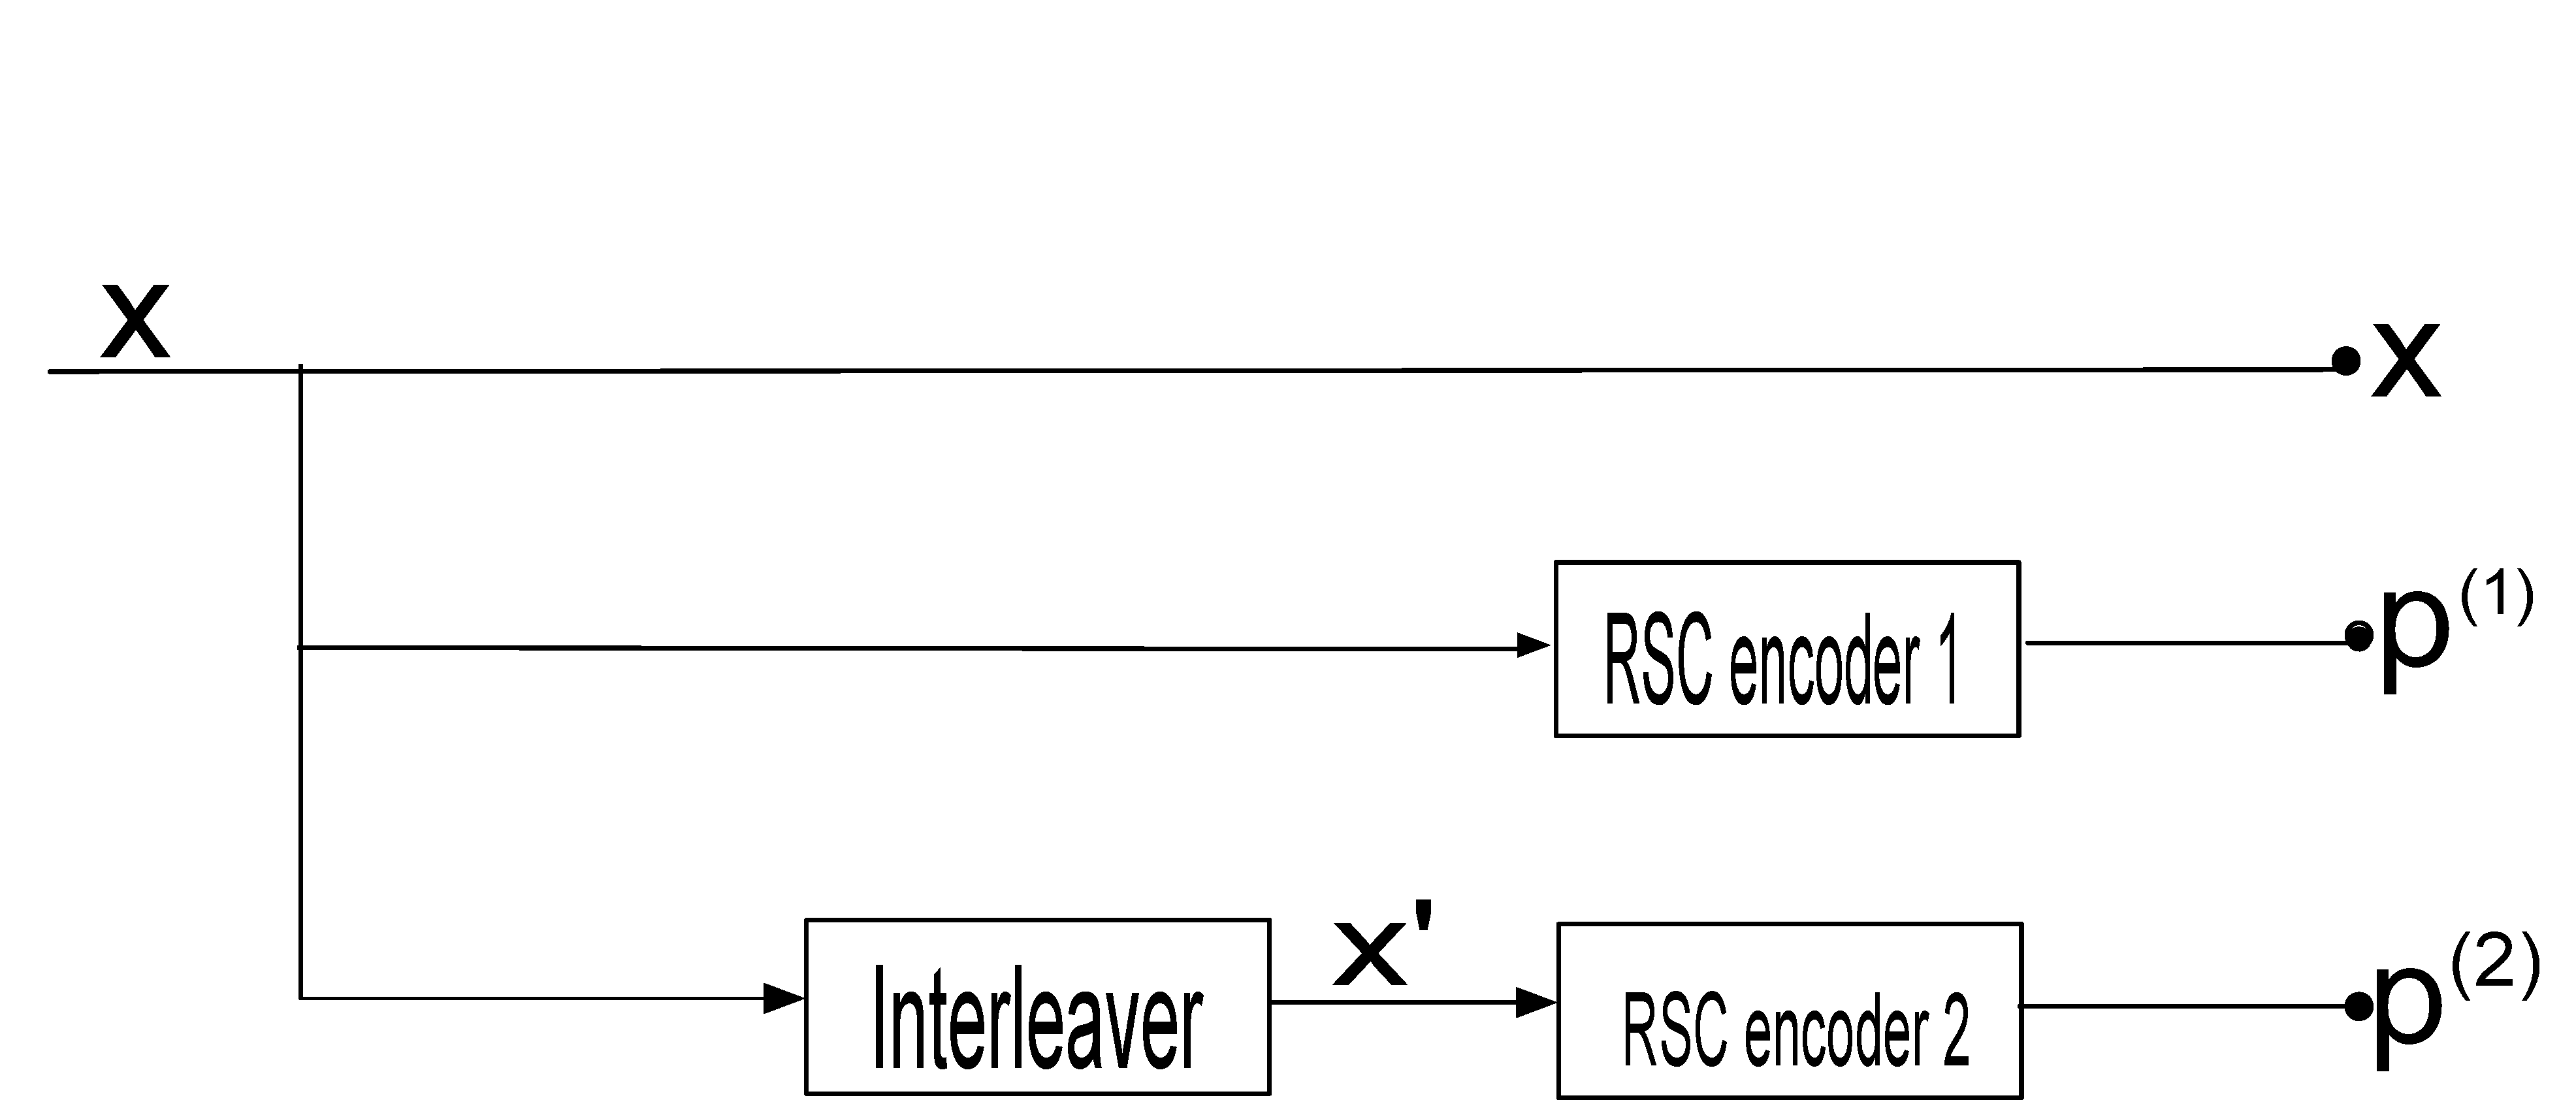
\includegraphics[height = 4cm, width=0.65\textwidth]{TurboEncoder.eps}
	\end{figure}

%\begin{figure}%[h!]
%\centering
%		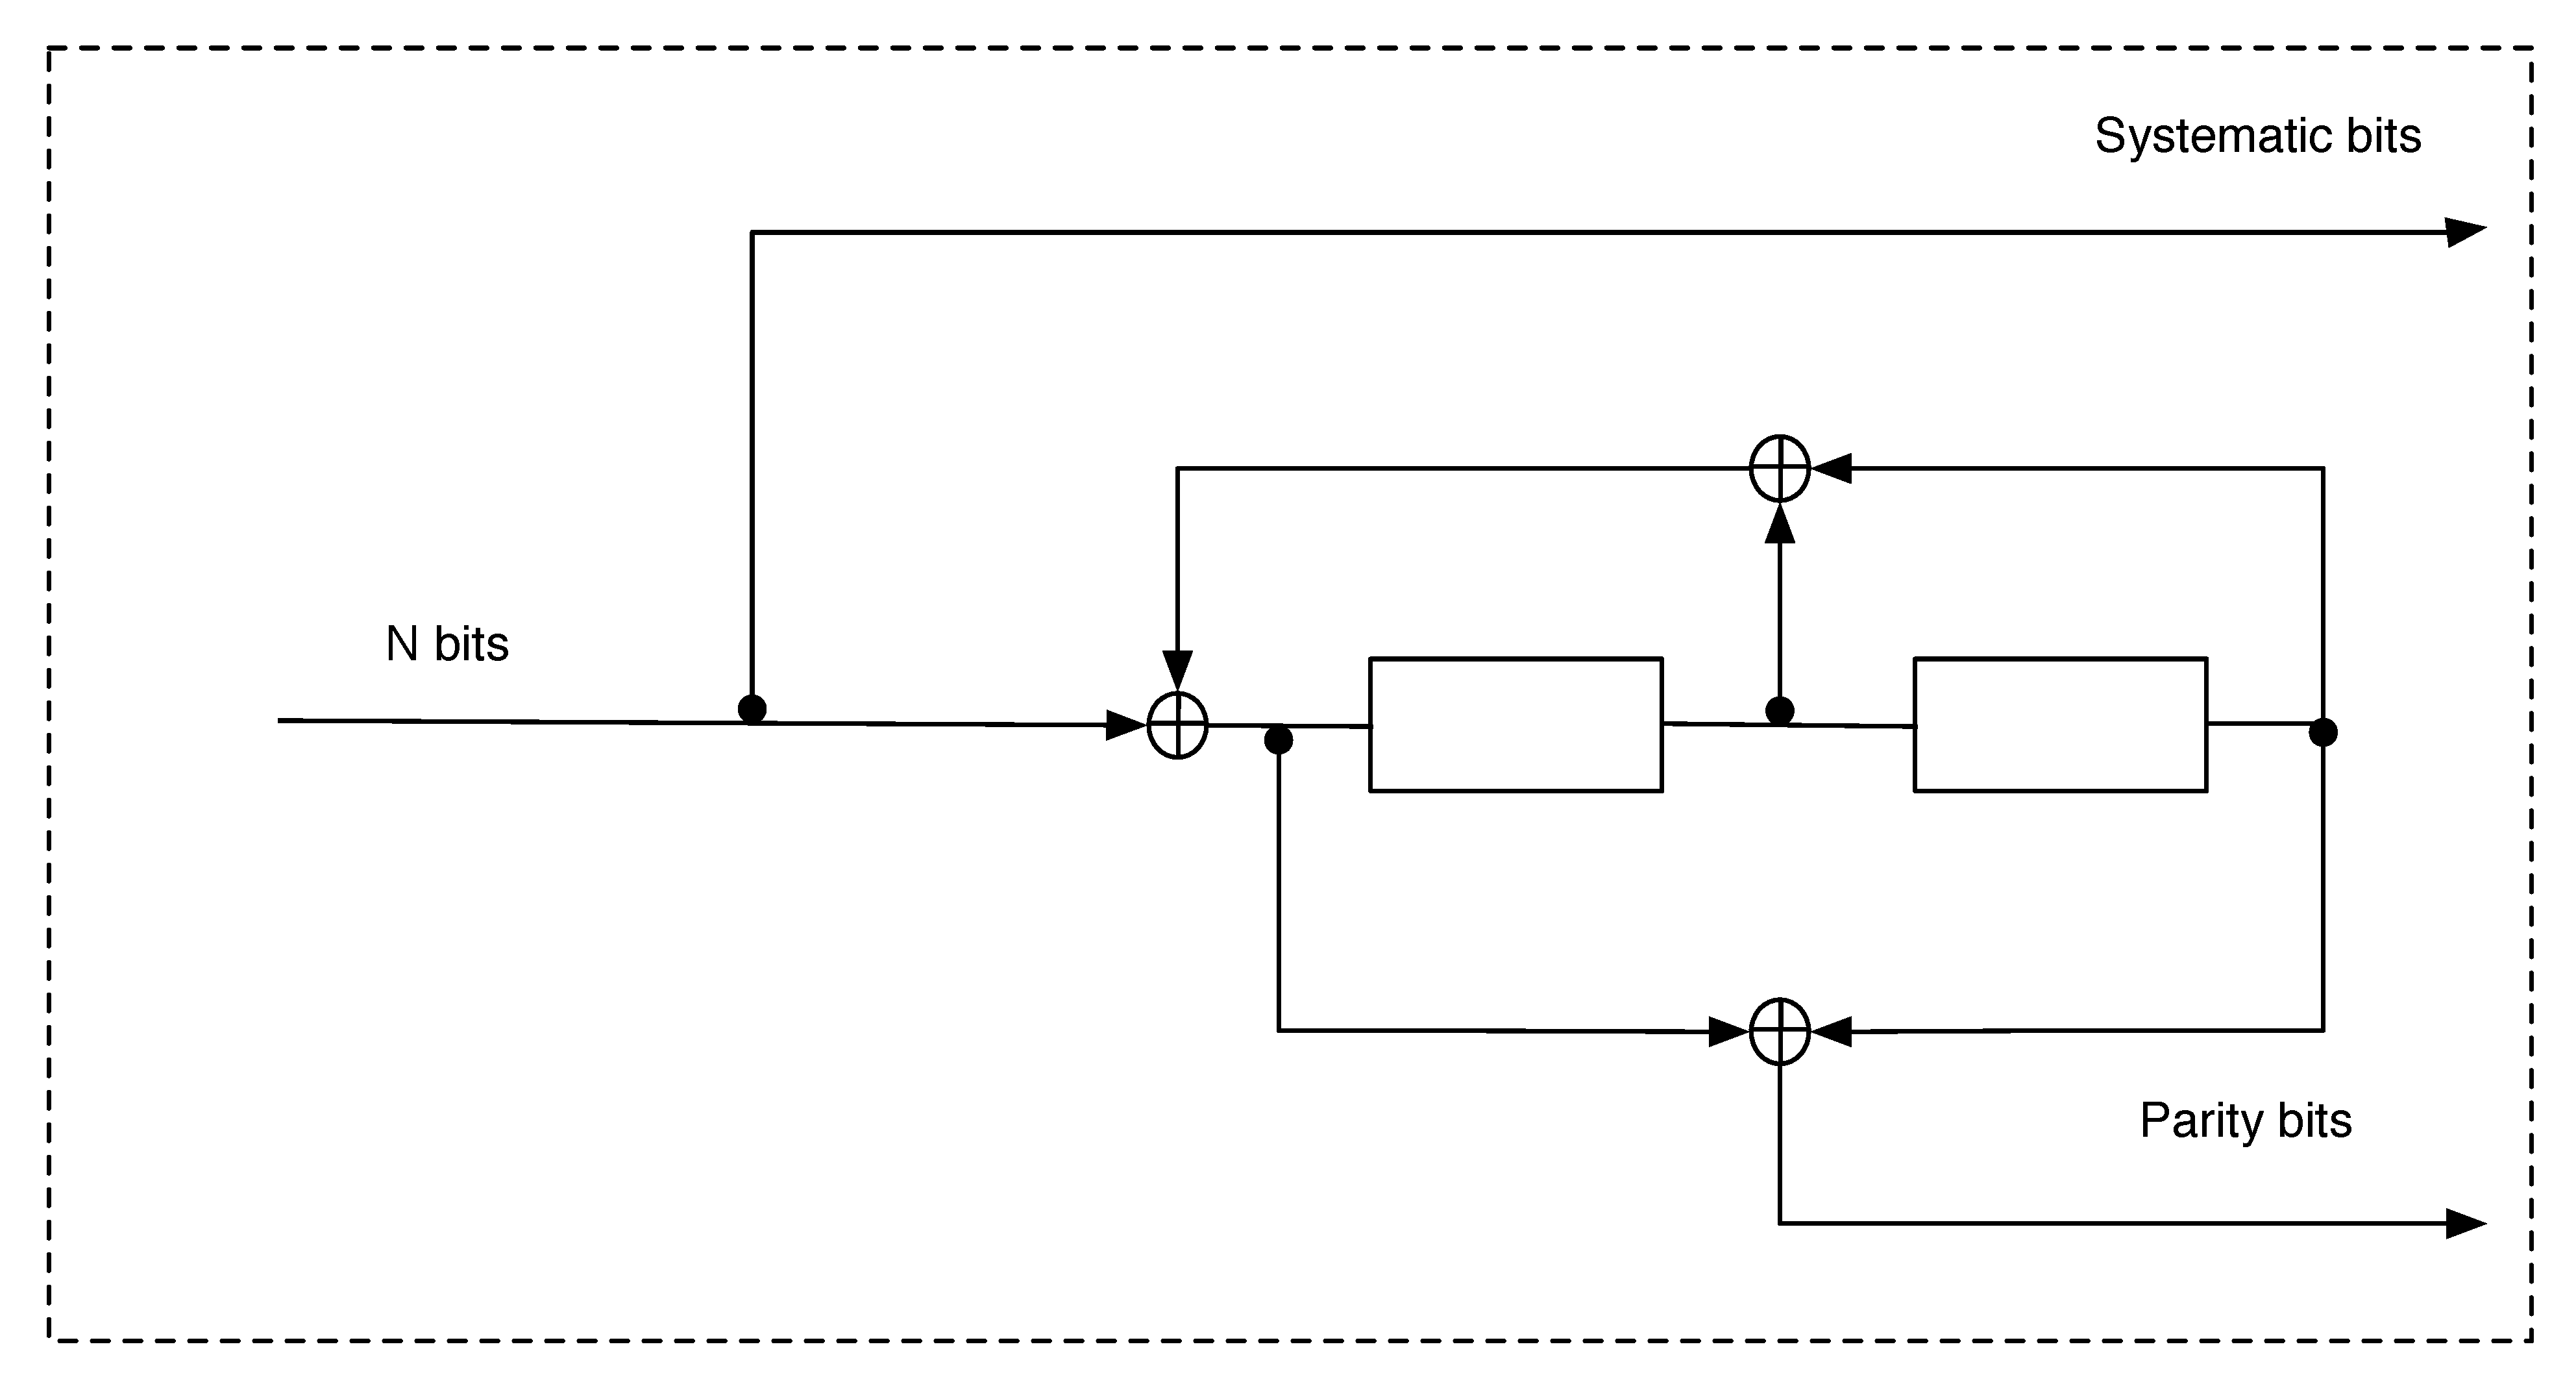
\includegraphics[width=0.55\textwidth]{RSCExample3.pdf}
		%\caption{$[\frac{1+D^2}{1+D+D^2}]$  RSC Encoder}
	%	\label{RSC}
	%	\end{figure}

%\blfootnote{N: Interleaver size, M: No. of memory elements}
\begin{itemize}
\item N is interleaver size, M is No. of memory elements
\item $\mathbf{x}$ is information bits with length $N-M$
\item $\mathbf{p}^{(1)}$ is upper parity checkbits, $\mathbf{p}^{(2)}$ is lower parity checkbits 

\begin{itemize}
\item both have length $N$
\end{itemize}

\end{itemize}

\end{frame}



%slide 5
\begin{frame}
\frametitle{5. Turbo Decoder}

\begin{figure}
\centering
		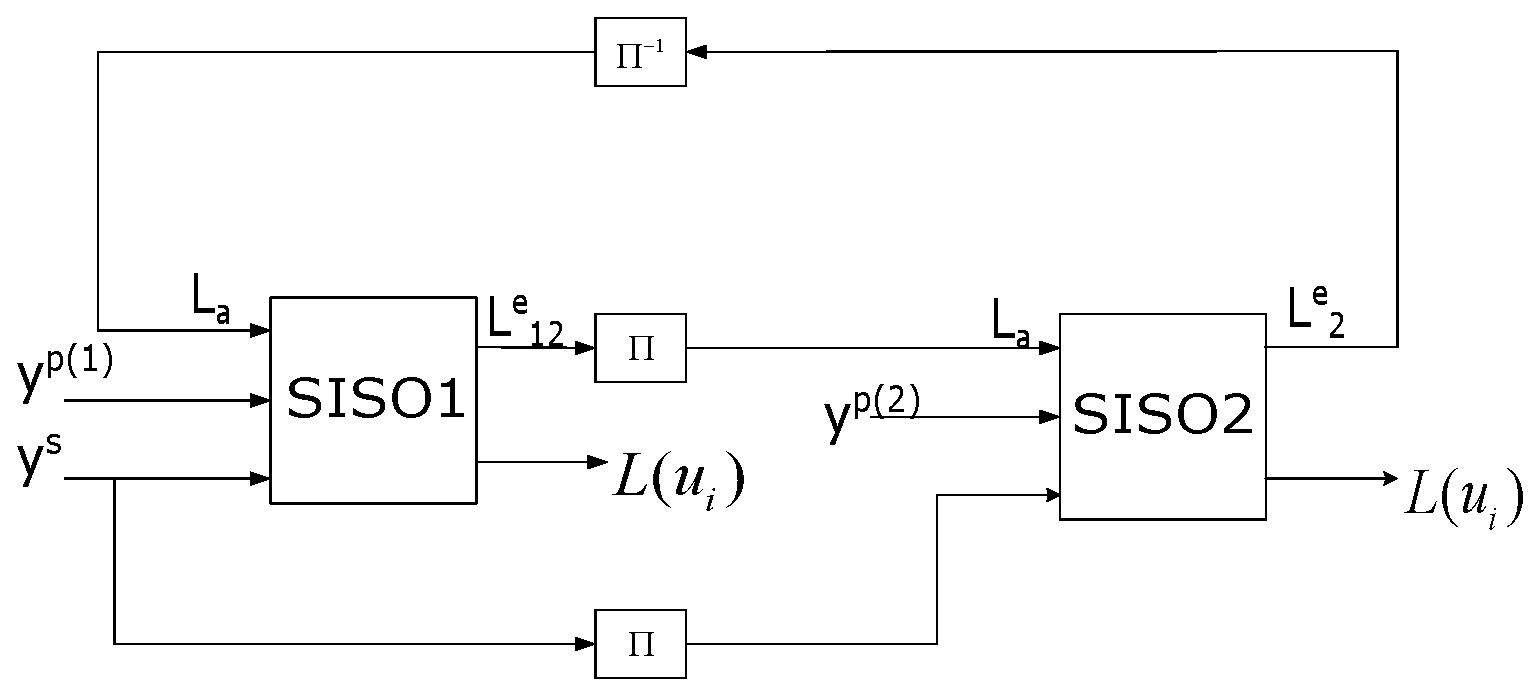
\includegraphics[width=8.5cm]{D1.eps}
	\end{figure}
\begin{itemize}
\item $y^s$ is systematic bits

\item $y^{p(1)}$ is upper parity check bits,  $y^{p(2)}$ is lower parity check bits

%\item $y^{p'}$ : lower parity check bits

\item $L(u_i)$ is Log-Likelihood Ratio, $L^e_{12}, L^e_{21}$ is extrinsic information

%\item 
\end{itemize}

\end{frame}

%Slide 6
%\subsection{$\tau$-seperated weight 2m errors}
\begin{frame}
\frametitle{6. RSC Encoders }
\begin{itemize}
\setlength\itemsep{2em}

\item cycle length ($\tau$) of RSC encoders
\begin{itemize}
\item length of the cycle with input $[1, 0, 0, 0, 0,...]$
\end{itemize}

\begin{example} 
\begin{columns}



%\centering
%$\Big[\frac{1+D^2}{1+D+D^2}\Big]$ (5/7)  RSC Encoder
\column{0.55\textwidth}
\begin{figure}%[h!]
%\centering
		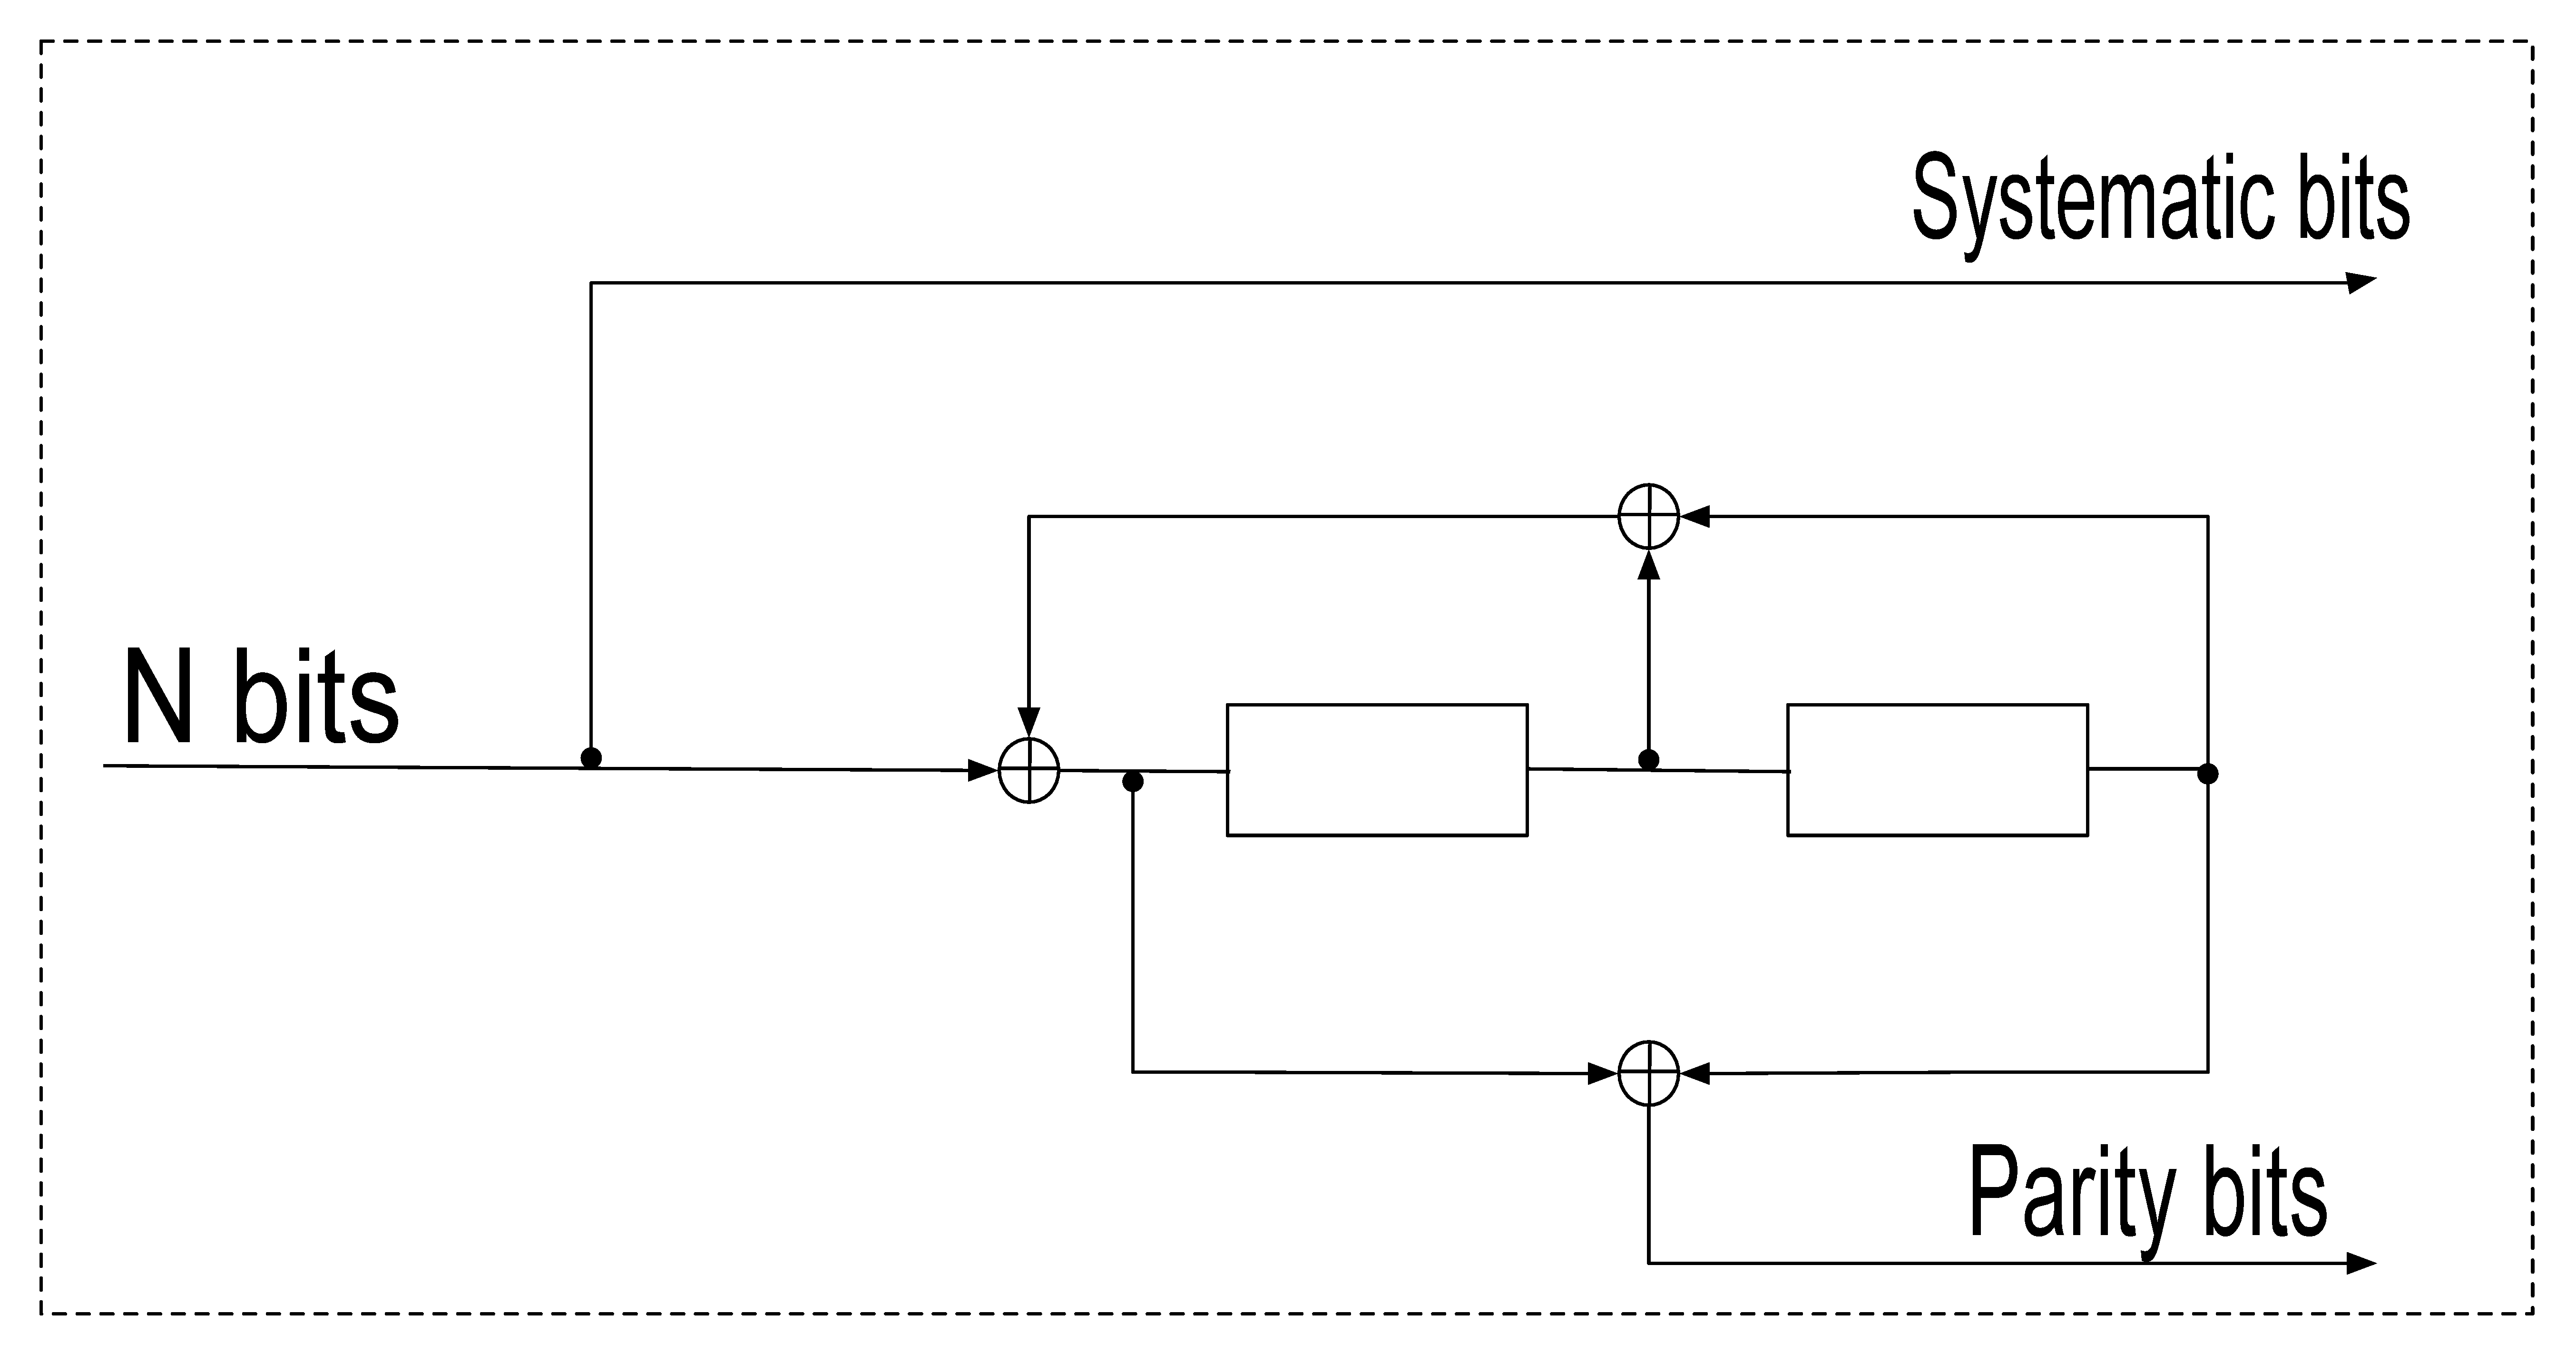
\includegraphics[height = 4.5cm, width=\textwidth]{RSCExample3.eps}
		%\caption{$[\frac{1+D^2}{1+D+D^2}]$  RSC Encoder}
		\label{RSC}
		\end{figure}
\column{0.45\textwidth}
\begin{itemize}
%\setlength\itemsep{2em}
\item $\Big[\frac{1+D^2}{1+D+D^2}\Big]$ (5/7)  RSC Encoder
 \item output : $[1,|1,1,0|,|1,1,0|,|1,1,0|...]$ 

 \item cycle : $[1,1,0]$ , $\tau = 3$

\end{itemize}

\end{columns}
\end{example}



\end{itemize}

\end{frame}

%Slide 9
%\subsection{$\tau$-seperated weight 2m errors}
\begin{frame}
\begin{itemize}
 
\setlength\itemsep{2em}

\frametitle{7. RSC Encoders and $a\tau$-seperated weight 2 errors}

\item weight $2$ information sequences 
\begin{itemize}
\item "1" bit pair seperated by $a\tau -1$ "0" bits
\end{itemize}

\item effective free distance $d_{eff}$
\begin{itemize}
\item minimum codeword weight due to weight 2 input
\end{itemize}

\begin{example}
\centering
 $N=16$, input=$[1, 0, 0, 1,.....,0]$
\begin{figure}
		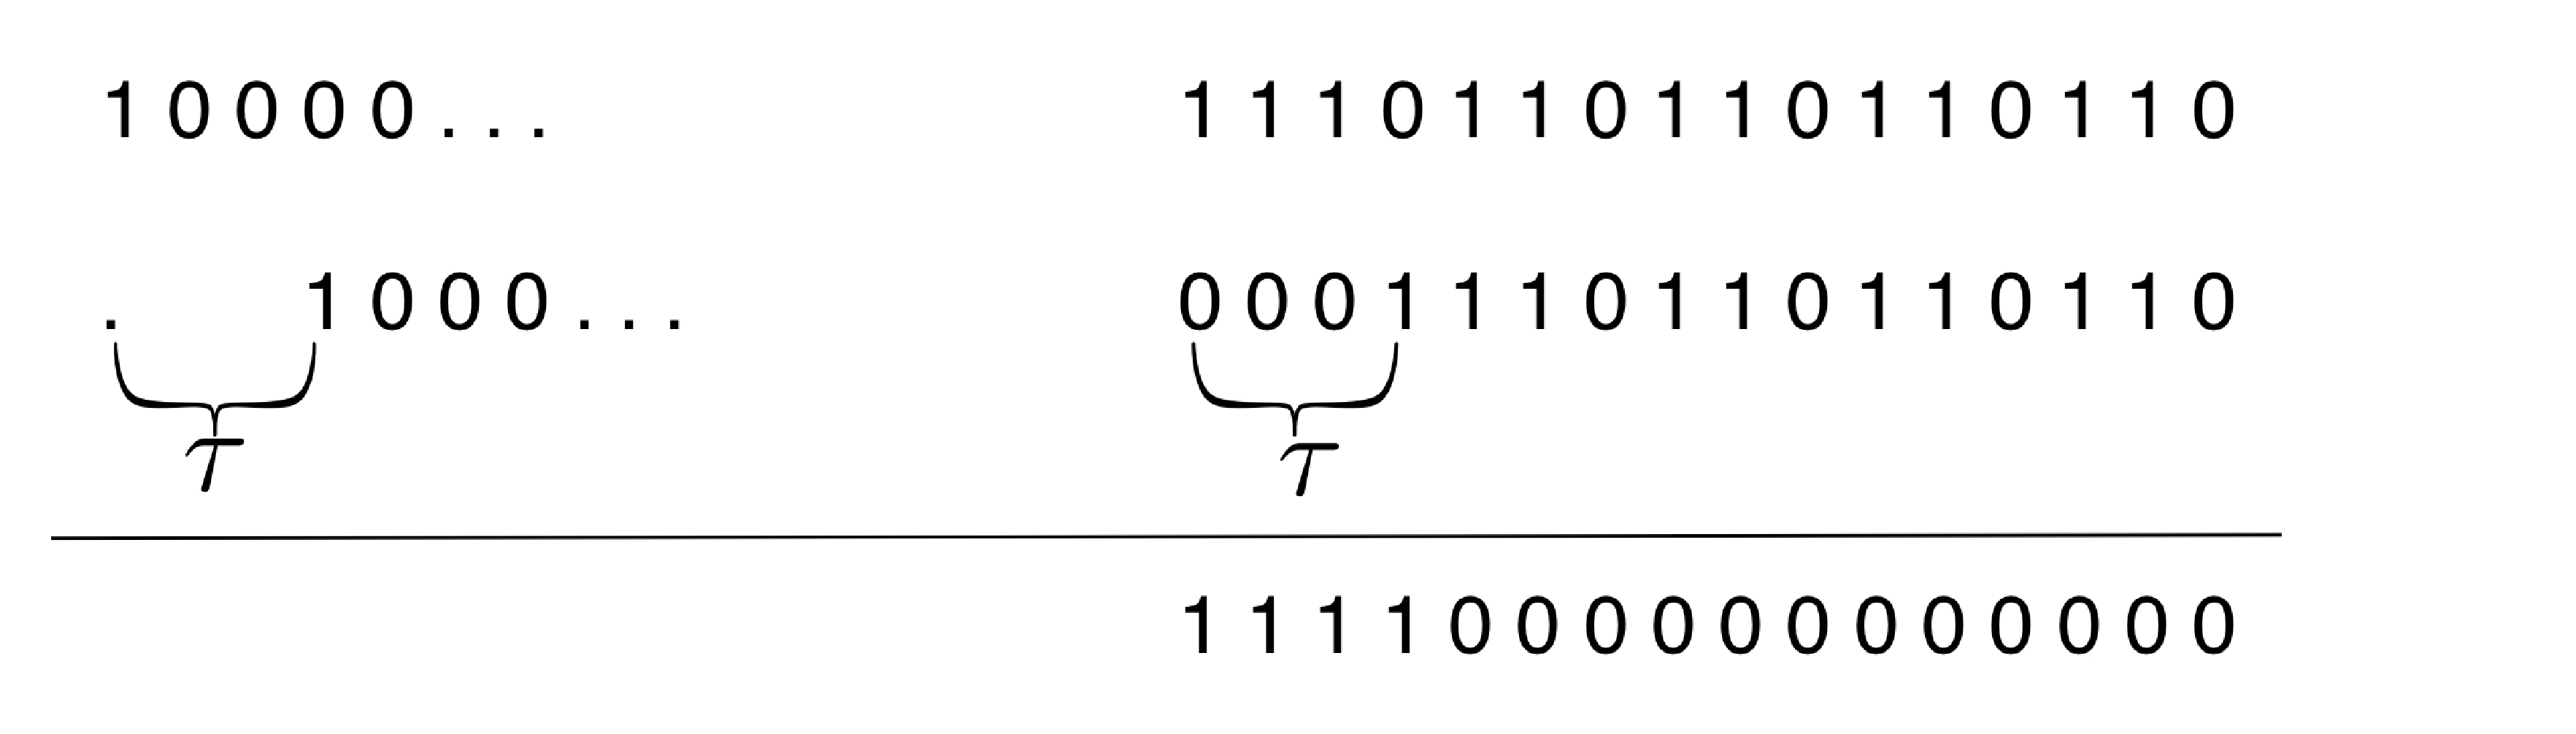
\includegraphics[width=0.95\textwidth]{RSCExample.eps}
		
	\end{figure}
\end{example}
\item  \textcolor{red}{low-weight  codewords}.


\end{itemize}

\end{frame}

%Slide 10
\begin{frame}
\frametitle{8. $t$-seperated weight 2 error in Turbo Codes}


\begin{center}
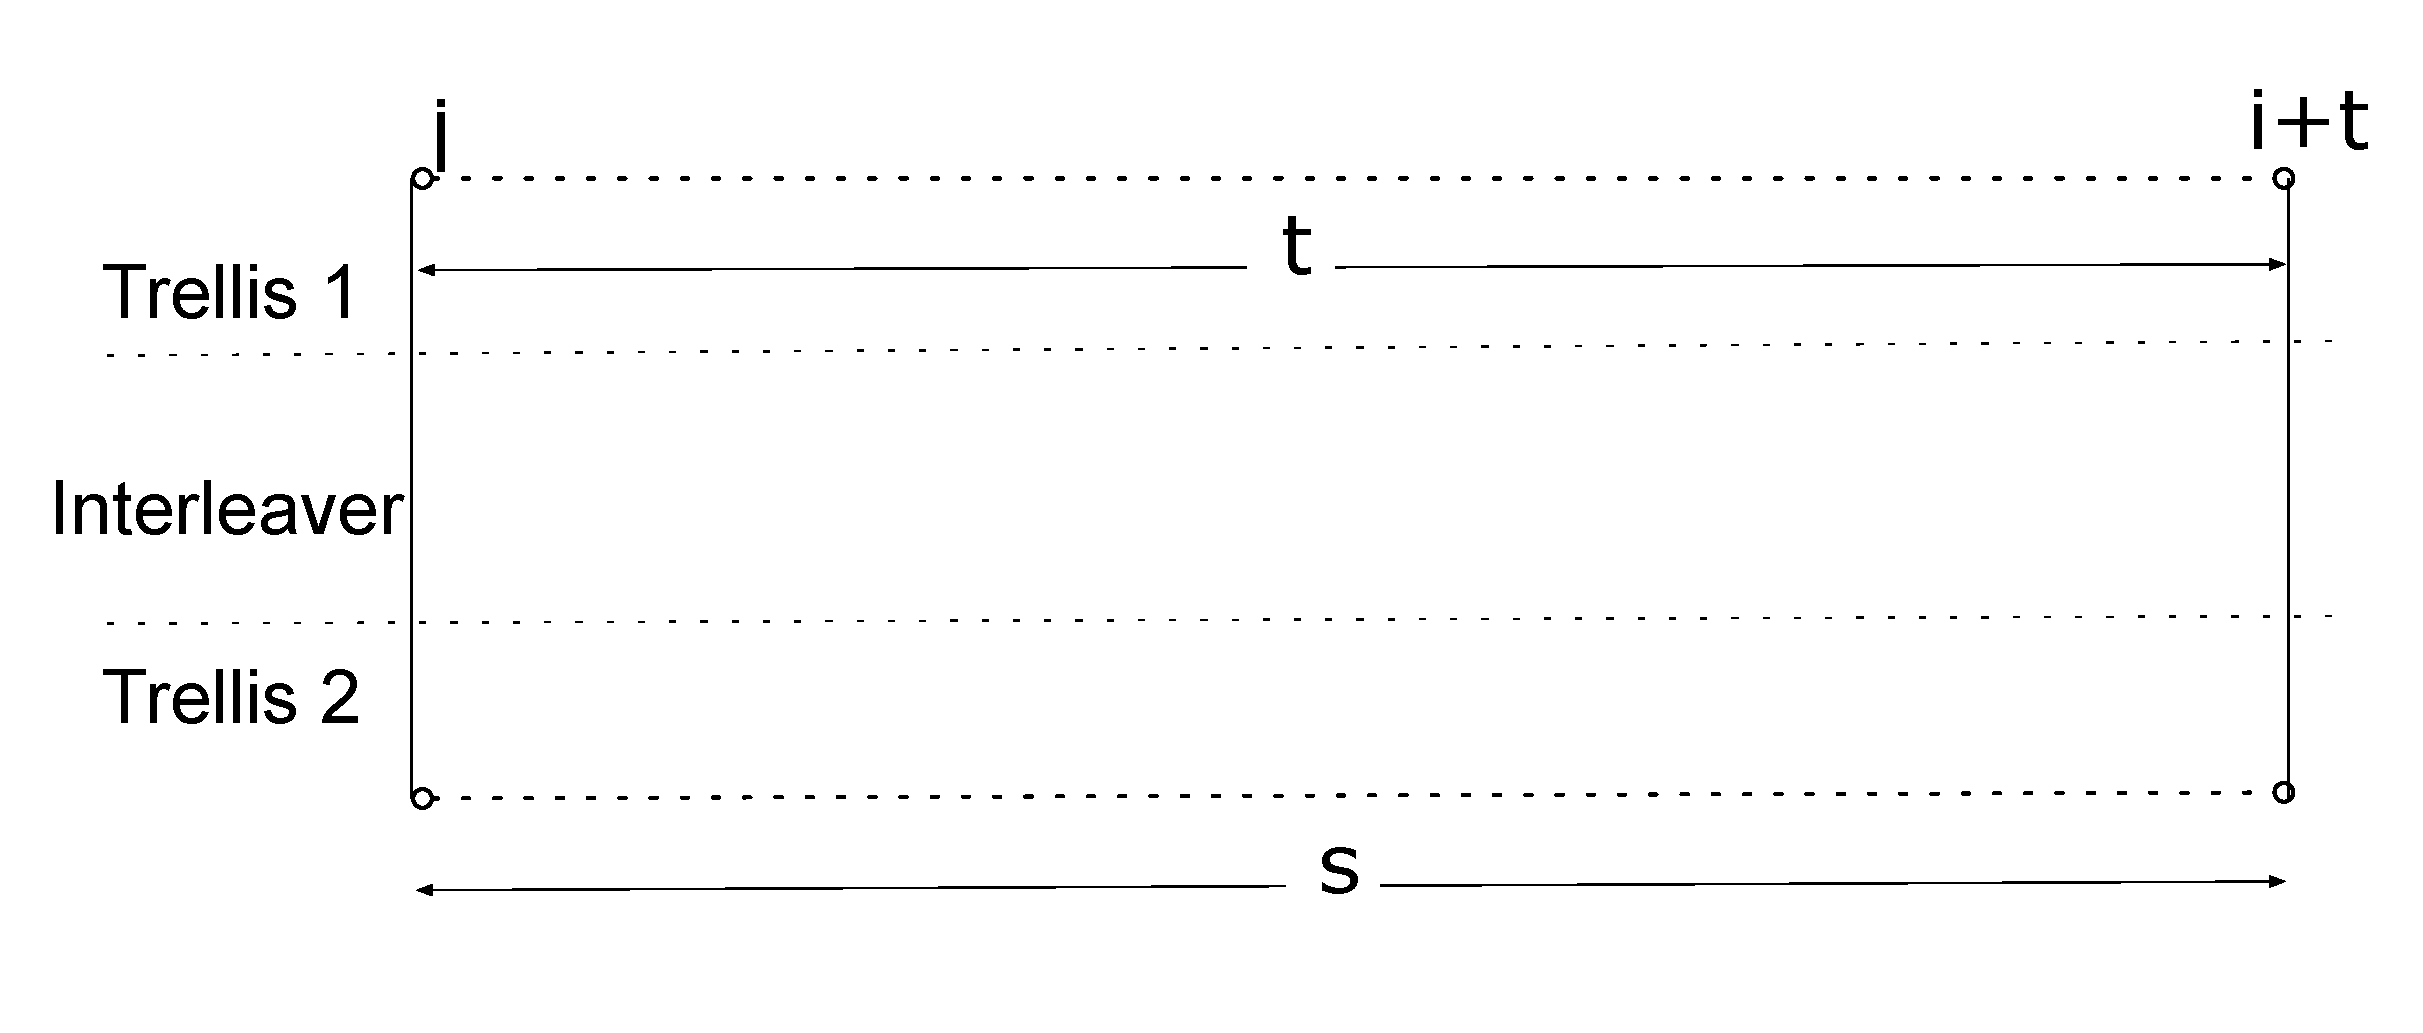
\includegraphics[width=0.8\textwidth]{weight2.eps}
\end{center}

\begin{itemize}
\item 
$t=a\tau
\mapsto s=b\tau$,
 \textcolor{red}{low-weight turbo codewords}.
 \end{itemize}
\end{frame}

%%%%%%%%%%%%%%%%%%%%%%%%%%%%%%%%

\begin{frame}
\frametitle{9. $\tau$-seperated Weight 2 Error - based Parameter Optimization}

\begin{itemize}
\item Linear Interleaver with depth $D$

\begin{equation}
 \Pi_{\mathfrak{L}_N}(i) = Di \mod N,\,\,\,\,\, gcd(N,D)=1;
\end{equation}

\item input - output distance relationship
 \begin{equation} 
 s = Dt \mod N
 \label{cong}
 \end{equation}
 
 \item prevent $t=a\tau \mapsto s=b\tau$
 
\begin{itemize}
\item Solution: \textcolor{green}{$\min{ (a+b)}$ \,\,\,,$D$ with largest $\min{ (a+b)}$} 


\end{itemize}
\end{itemize}

\end{frame}


%Slide 11
\begin{frame}
\frametitle{10. $a\tau$ weight 2 error : Interleaver Search}
\begin{block}{Linear Interleaver Search Results}
\begin{table}[h!]
\centering
\begin{tabular}{||c |c |c |c |c |c ||} 
 \hline
 $D$ & 13 & 121 & 17 & 23 & 21\\ [0.5ex] 
 \hline\hline
 $a $ & 19 & 17 & 15 & 11 & 12 \\ 
 \hline
  $b $ & 9 & 9 & 1 & 3 & 4 \\ 
  \hline
  $d_{eff} $ & 30 & 30 & 15 & 26 & 15 \\ 
  \hline
  $N_{free}$ & 1 & 1 & 2 & 1 & 2 \\ [1ex] 
 \hline
\end{tabular}
\label{tab1}
\end{table}
\end{block}

\begin{block}{ BER Approximation}


\begin{equation} 
 P_b \approx \frac{1}{2}\sum_{w_c}D_{w_c} 
  erfc \Bigg(\sqrt{w_c\frac{R_cE_b}{N_o}} \Bigg)
  \label{aprox}
  \end{equation}
  
 where 
  $$ D_{w_c}\triangleq \sum_{w_x+w_p=w_c} \frac{w_x}{N}A_{w_x,w_p}$$
  %$w_x$ is the weight of the input sequence, $w_p$ is the weight of the parity 
  %sequence,$R_c$ is the rate of the turbo code , $w_c$ is the weight of the turbo 
  %codeword and $A_{w_x,w_p}$ is the multiplicity of $w_c$.
\end{block}
\end{frame}


%%%%%%%%%%%%%%%%%%%%%%%%%%%%%

%Slide 11
\begin{frame}
\frametitle{11. BER Approximation vs Simulation}

\begin{tikzpicture}[remember picture,overlay]
            \node[at=(current page.center)] {
                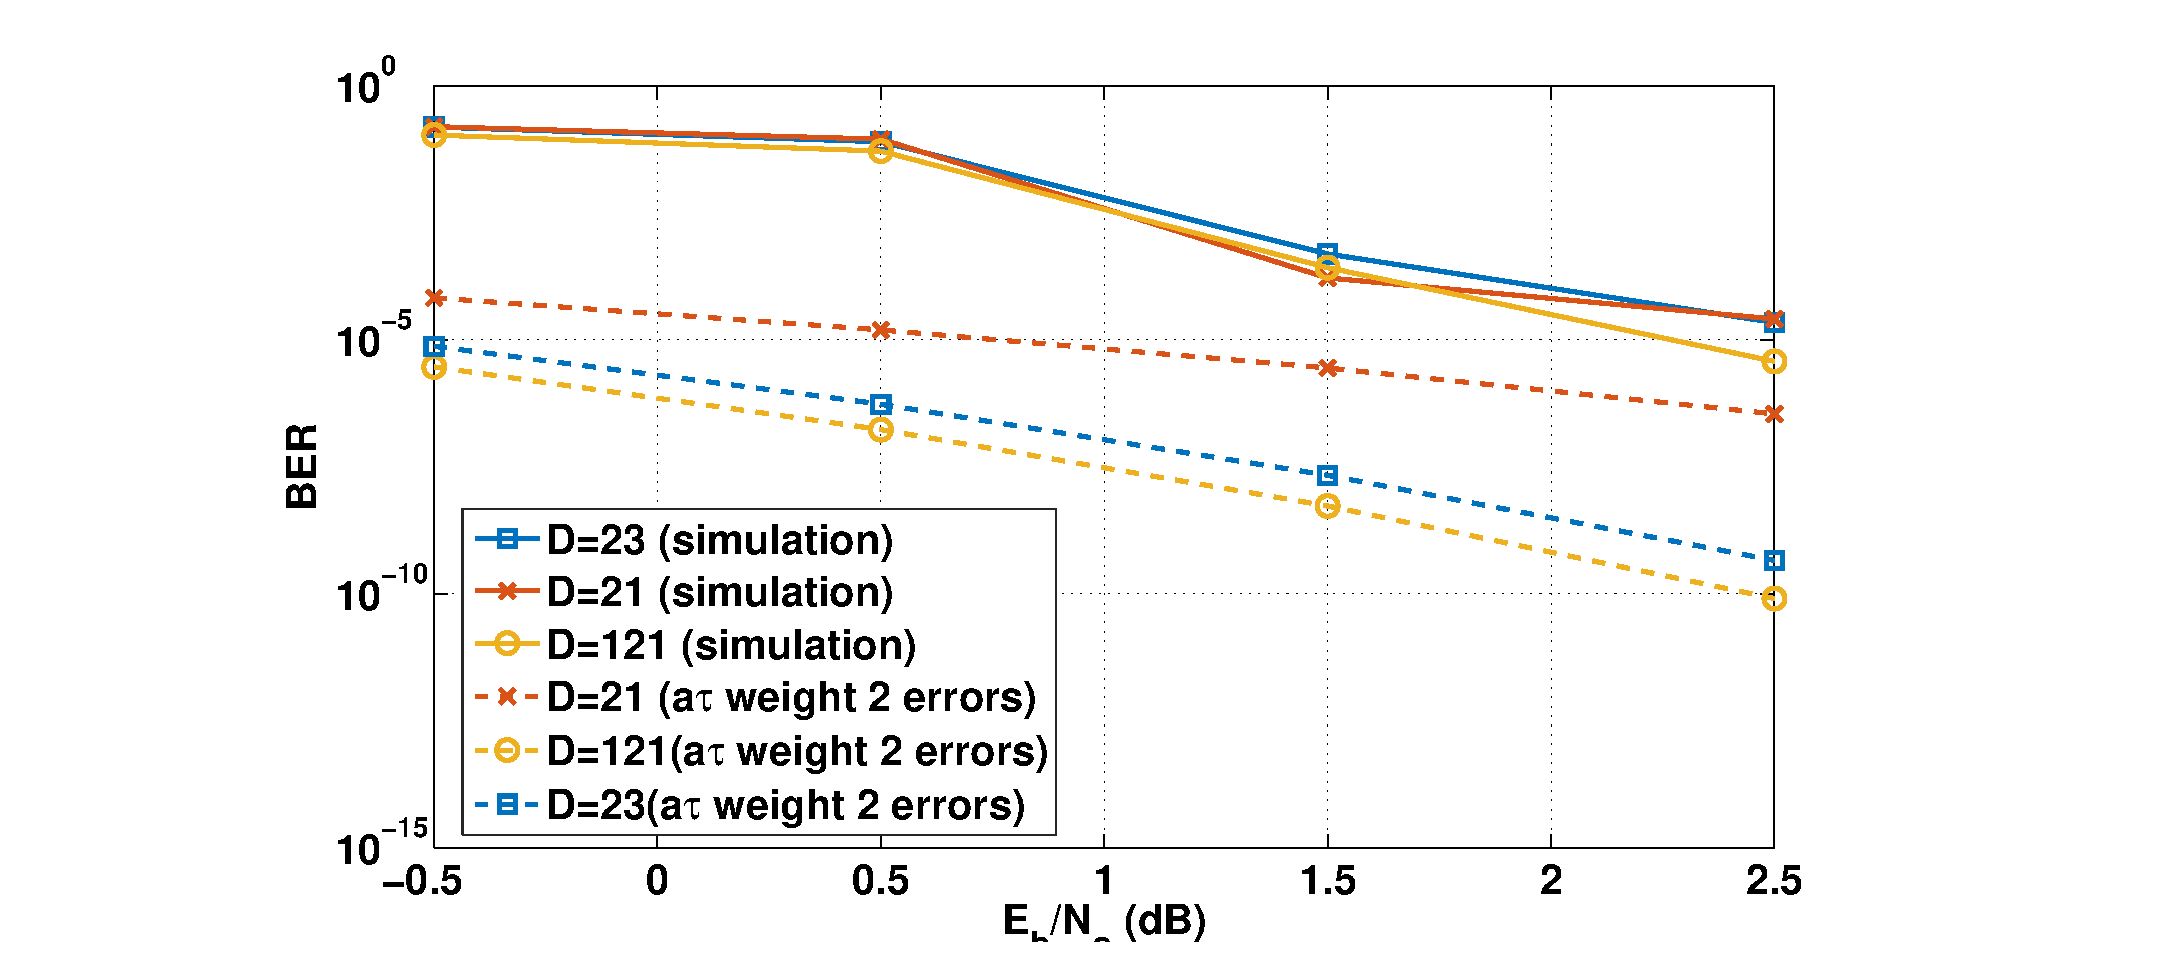
\includegraphics[height = 8cm,width=1.40\paperwidth]{D_23_21_121_N_256.eps}
            };
        \end{tikzpicture}



\end{frame}


%%%%%%%%%%%%%%%%%%%%%%%%%%%%%
%Slide 11
\begin{frame}
\frametitle{12.  $\tau$-seperated weight 4 errors}
\begin{itemize}
\item Dominate BER performance [2]
\begin{center}
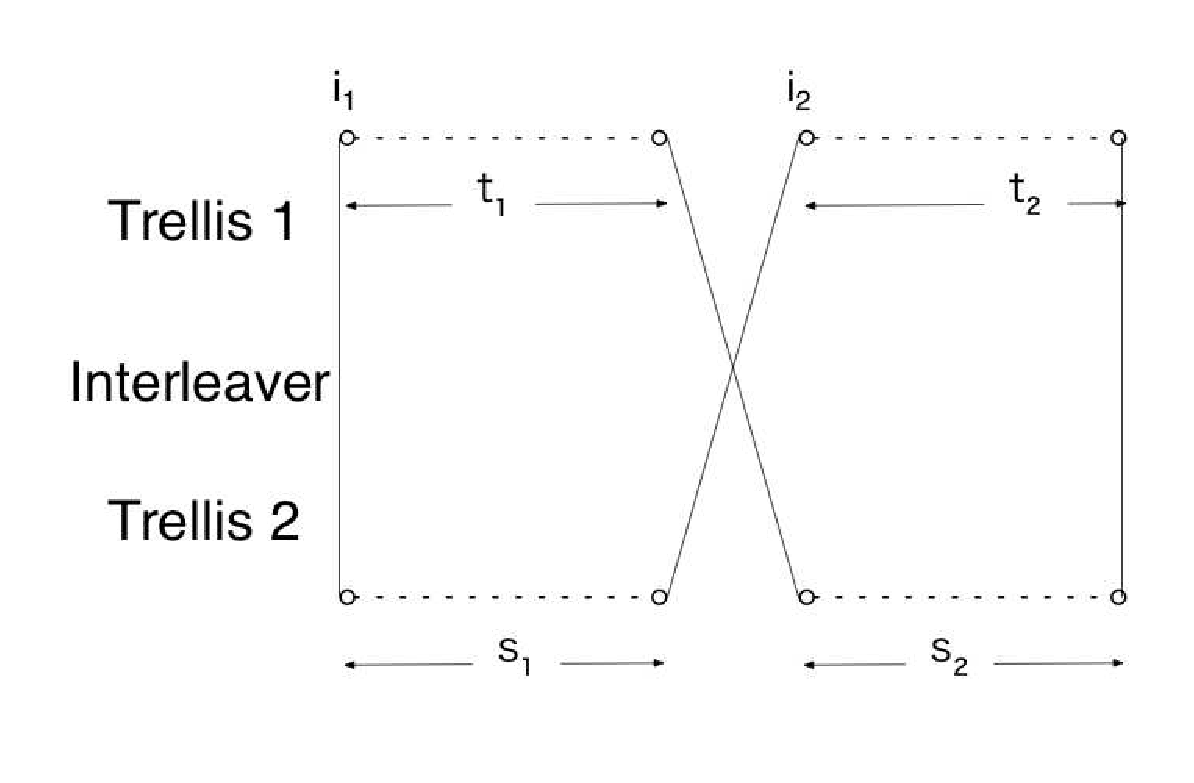
\includegraphics[height = 4.5cm,width=0.8\textwidth]{weight4.eps}
\end{center}


\item Weight $4$ input :$ (1+D^v)(1+D^{\tau})$

\begin{itemize}
 \item $\tau = Dv  \mod N$
\end{itemize}

\end{itemize}
\blfootnote {[2] Oscar Y. Takeshita, Member, IEEE, and Daniel J. Costello ,
''New Deterministic Interleaver Designs for Turbo Codes'',IEEE Trans. Inform. 
Theory, vol.  46,pp. 1988-2006,Nov. 2000}
\end{frame}
%%%%%%%%%%%%%%%%%%%%%%%%%%%%%%%



%%%%%%%%%%%%%%%%%%%%%%%%%%%%%%%
\begin{frame}
\frametitle{12.  $\tau$ weight 4 errors}


\begin{example}
\begin{itemize}
\item  $N=32,\, \tau=3, \, D=5,\, v=7$

\item input : $(1+D^3)(1+D^7)$  , output :$(1+ D^3)(1+D^{15})$

\end{itemize}
\end{example}

\begin{itemize}
\setlength\itemsep{2em}
\item codeword weight : $20$, multiplicity $\approx N$

\item same results for different $D$ and $N$
\end{itemize}




\end{frame}
%%%%%%%%%%%%%%%%%%%%%%%%%%%%%%%%%%%%

%Slide 11
\begin{frame}
\frametitle{13.  $\tau$ weight 4 error : BER Approximation vs Simulation}

\begin{tikzpicture}[remember picture,overlay]
            \node[at=(current page.center)] {
                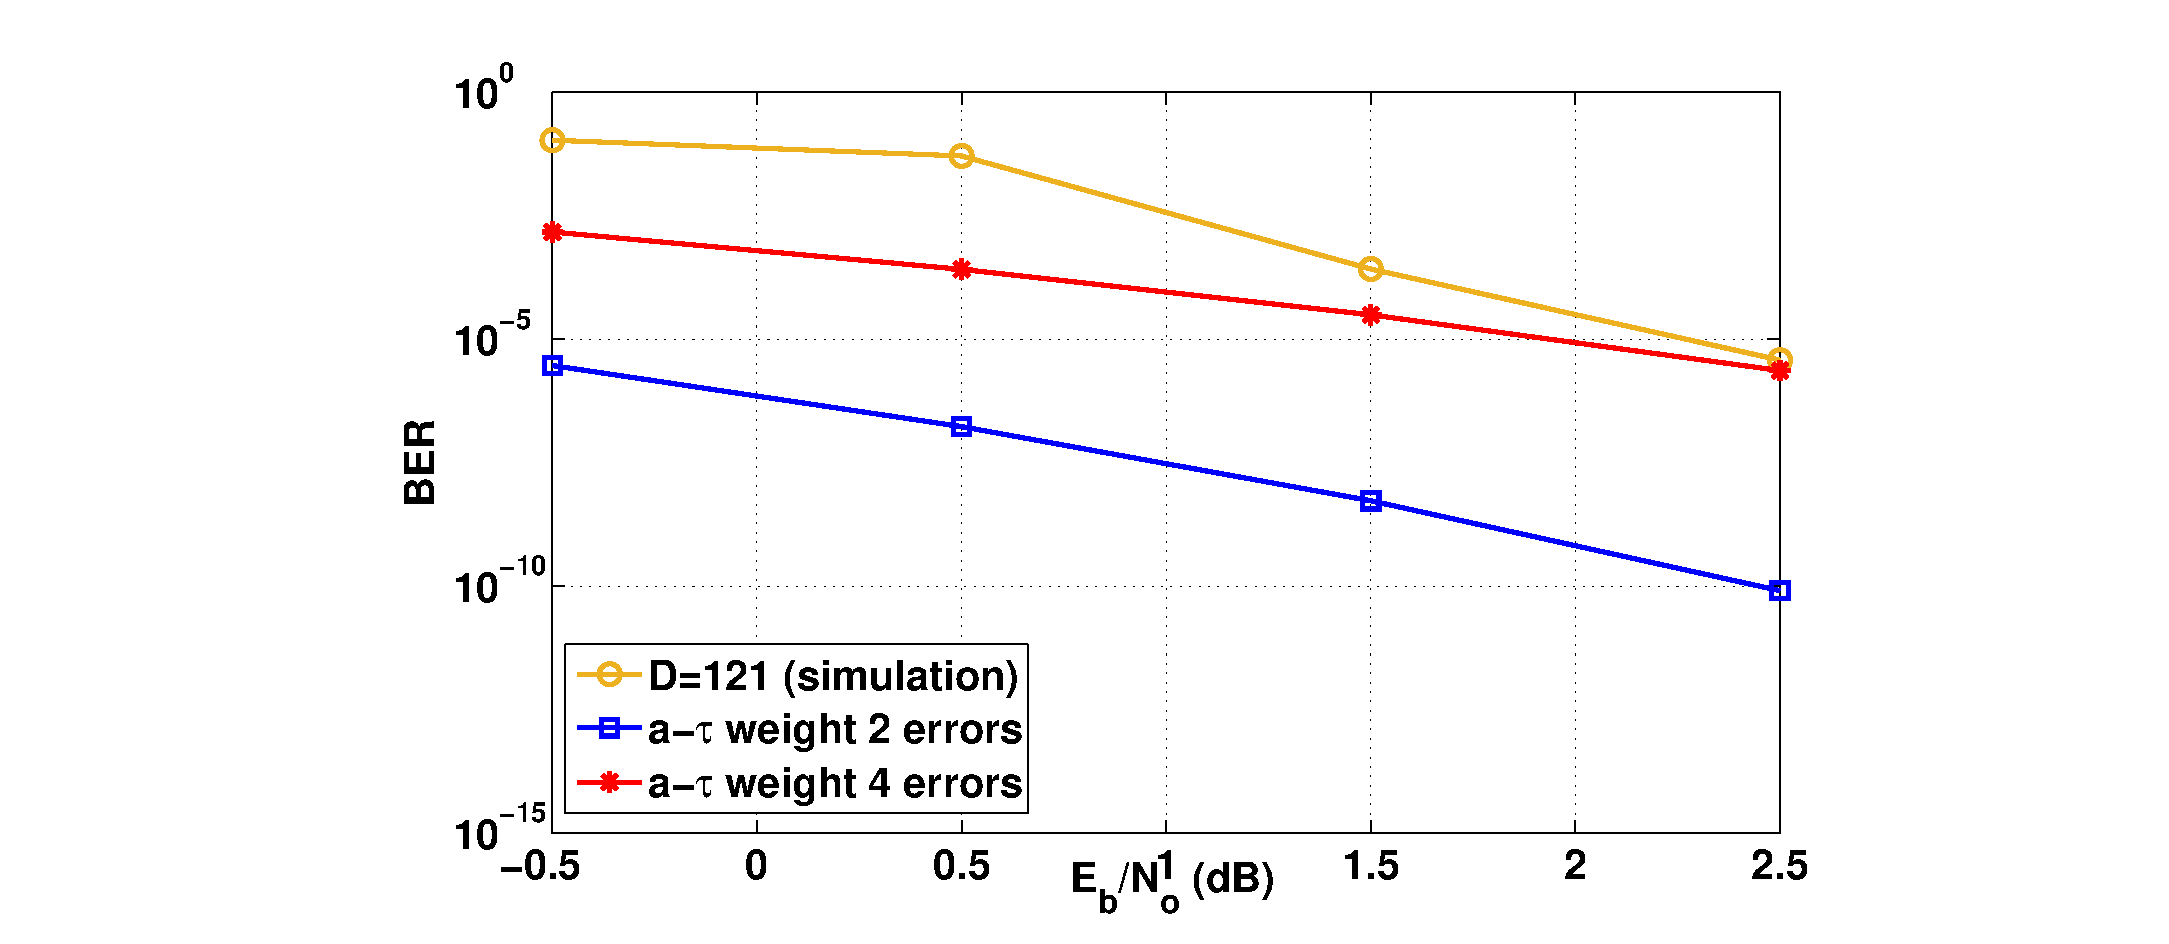
\includegraphics[height = 8cm,width=1.45\paperwidth]{D_121_N_256_sim_vs_theory.eps}
            };
        \end{tikzpicture}


\end{frame}


%%%%%%%%%%%%%%%%%%%%%%%%%%%%%%%%%%
%Slide 12
\begin{frame}
\frametitle{14. Sequential representation of Linear Interleaver}

\begin{itemize}
\setlength\itemsep{2em}
%\item $d_{ef}$: 2エラーイベントの入力による、符号語の最低距離

\item Weight 4 error dominates performance

 \item Algorithm for linear interleaving



\begin{itemize}
\setlength\itemsep{1.5em}
\item 1. $p_0=0$
 
\item 2. $p_i=(p_{i-1}+\textcolor{red}{D}) \mod N$

\end{itemize}



\item element positions shifted  by constant $D$
\end{itemize}

\blfootnote{$p_i$ is element position}
\end{frame}
%Slide 13
\begin{frame}
\frametitle{15. Multi-Shift Interleaver}

\begin{itemize}
\setlength\itemsep{1.5em}



\item For $N=2^r,\,\,\, r\in \{ 1,2,...\}$ set $\Delta s= 2^q, \,\,\, q\in\{2,3,..,r-1\}$

\item cycle set $\mathbb{D}=\{d_0,d_1,...,d_{V-1}\},\,\,\, V=N/\Delta s$
\begin{itemize}
\item $d_i=d_{i-1}+\Delta s$
\end{itemize}

\item Algorithm for multi-shift interleaver

\begin{itemize}
\item 1. $p_0=0$
 
 \item 2. $p_i=p_{i-1}+\textcolor{red}{d_{((i-1) \mod V) } }\mod N,\,\,\,\,\,  \mathit{d_0 \,is \,an \,odd \,integer}$

\item Shift value of D for each position shift
\end{itemize}



%\item Algorithm in equation form:  $$\Pi_{\mathit{M}|{N:(d_0,\Delta s)}}(i)= \Big(  d_0 + \Delta s \frac{(i-1)}{2}\Big)i \mod N$$



\end{itemize}


\end{frame}



% slide 14
\begin{frame}
\frametitle{15. Multi-Shift Interleaver : Example}
\begin{example}
\begin{itemize}

\item original vector $$\mathbf{x}=[0, 1, 2, 3,...,31]$$
\setlength\itemsep{2em}
\item $N=32, \,\, \Delta s =4, \,\, d_0=5$ 
\begin{itemize}
\item $\mathbb{D}=\{5, 9, 13, 17, 21, 25, 29, 1\}$

\item 
\begin{equation*}
\begin{split}
\mathbf{p}= &[ 0, 5, 14, 27, 12, 1, 26, 23, 24, 29, 6, 19, 4, 25, 18, 15, 16, 21\\,
 &30, 11, 28, 17, 10, 7, 8, 13, 22, 3, 20, 9, 2, 31]
\end{split}
\end{equation*}
 \item interleaved vector:
\begin{equation*}
\begin{split}
\mathbf{x}'=&[0,5,30,27,12,1,10,23,24,29,22,19, 4, 25 ,2, 15,16, 21, 14, 11, 28\\,&17,
  26, 7, 8, 13, 6, 3, 20, 9, 18, 31]
\end{split}
\end{equation*}
\end{itemize}



\end {itemize}
\end{example}
\end{frame}




% slide 15
\begin{frame}
\frametitle{16. Optimal Parameter Search for Multi-Shift Interleaver}

\begin{itemize}
\setlength\itemsep{2em}

\item procedure for choosing good interleavers

\begin{itemize}
\setlength\itemsep{1em}
\item choose $d_0$ from $(\sqrt{N},N/2)$

\item calculate hamming weight for  $\Delta s \in 2^q$



\item best $\Delta s$ = largest $d_{eff}$



\item repeat for $d_0$ within range 

\item best parameter, $(d_0, \Delta s)$ with largest $d_{eff}$, least value of $\Delta s$ and multiplicity
\end{itemize}



\end{itemize}

\end{frame}

% slide 18
\begin{frame}
\frametitle{17.MSI Search Results : $5/7$ component encoder. $N=256$}
\begin{table}[h!]
\centering
\begin{tabular}{||c |c |c |c||} 
 \hline
 $d_0$ & 17 & 31 & 47 \\ [0.5ex] 
 \hline\hline
  $d_{eff}$ & 38 & 38 & 38 \\ 
 \hline
 $\Delta s$ & 64 & 128 & 64 \\ 
  \hline
  $N_{free, eff}$ & 207 & 208 & 209 \\ [1ex] 
 \hline
\end{tabular}
%\caption{ $5/7$,  component encoder. $N=256$}
\label{tab1}
\end{table}

\begin{itemize}
\item best parameter $(d_0=17,\Delta s = 64)$
\end{itemize}
\blfootnote{ $N_{free, eff}$ : multiplicity of $d_{eff} $codewords}
\end{frame}

% slide 19
\begin{frame}
\frametitle{17. Simulation Results for Table }
\begin{tikzpicture}[remember picture,overlay]
            \node[at=(current page.center)] {
                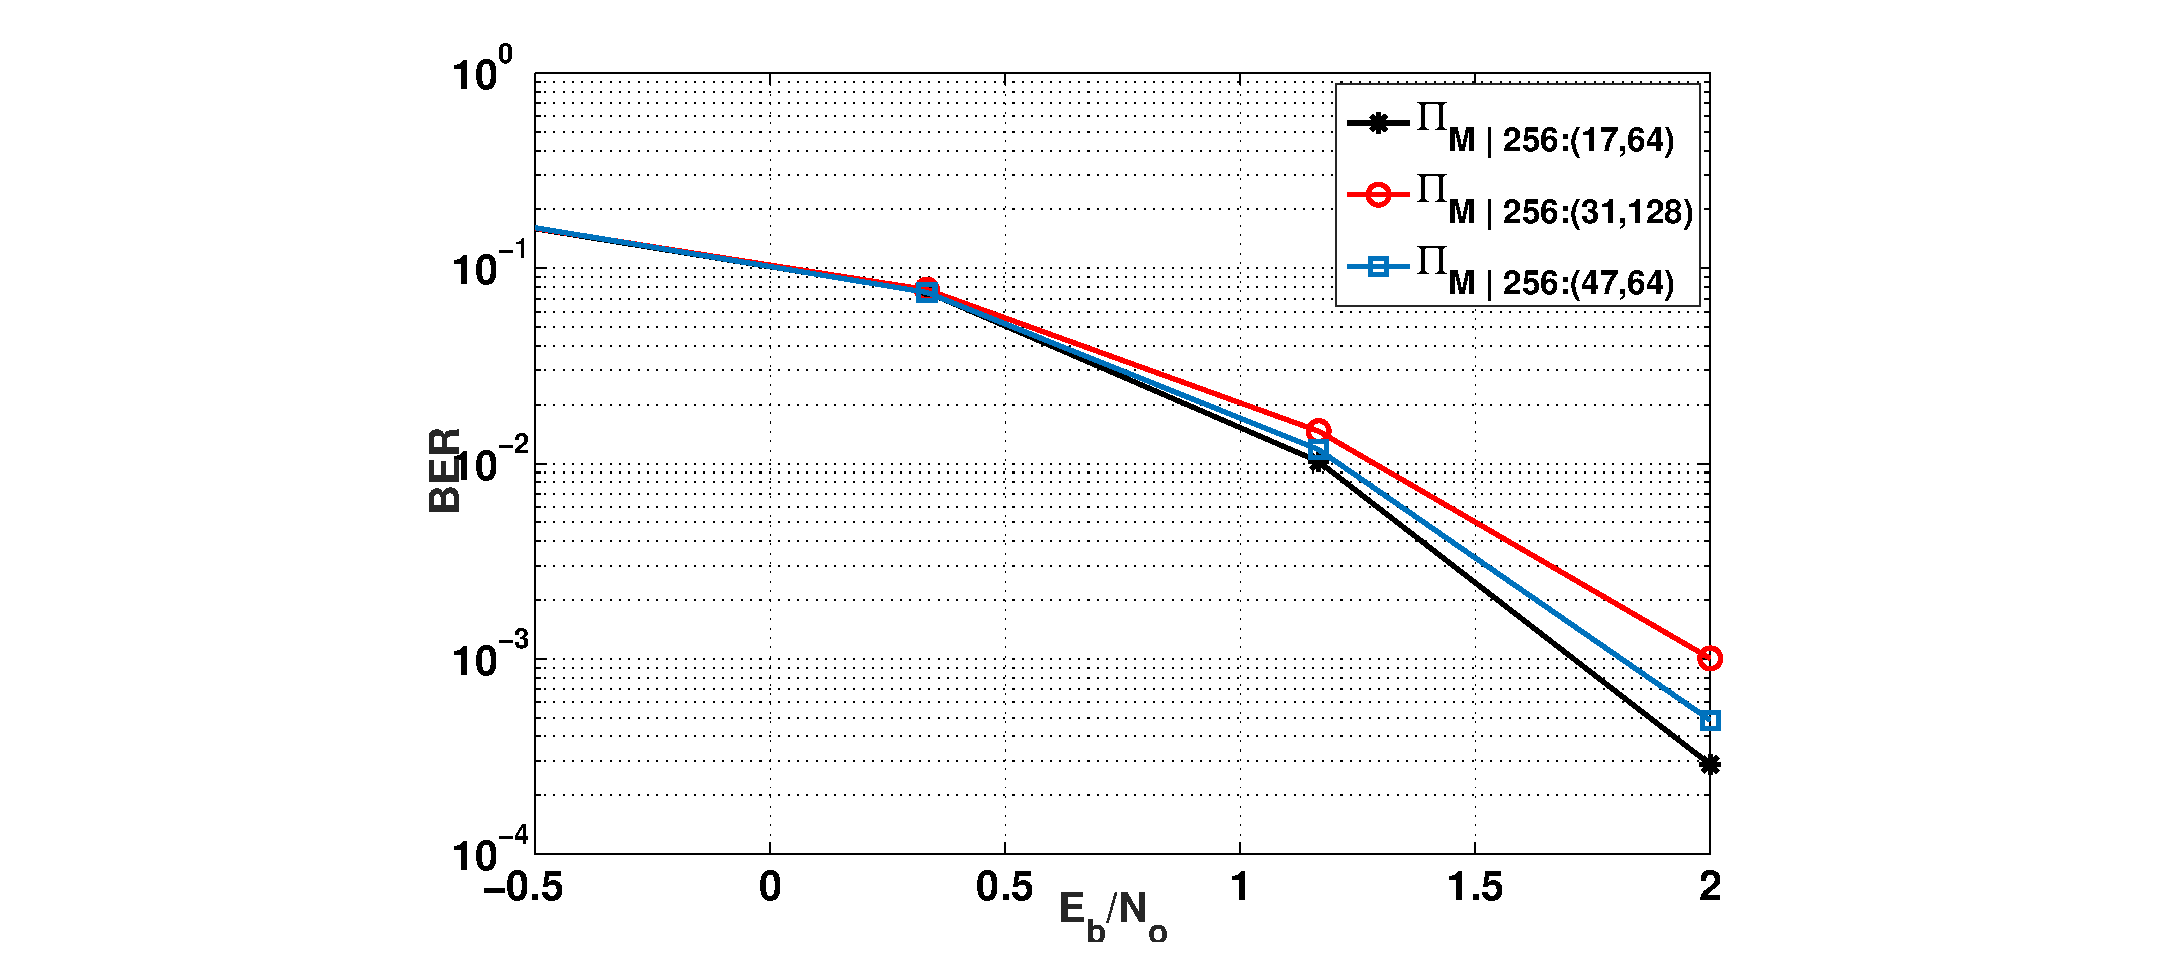
\includegraphics[width=1.35\paperwidth]{myInterleaver_(comparison_256)_5_7_3.eps}
            };
        \end{tikzpicture}

\end{frame}

% slide 20
\begin{frame}
\frametitle{17. Results for $5/7$ Component Code. $N=1024$}
\begin{tikzpicture}[remember picture,overlay]
            \node[at=(current page.center)] {
                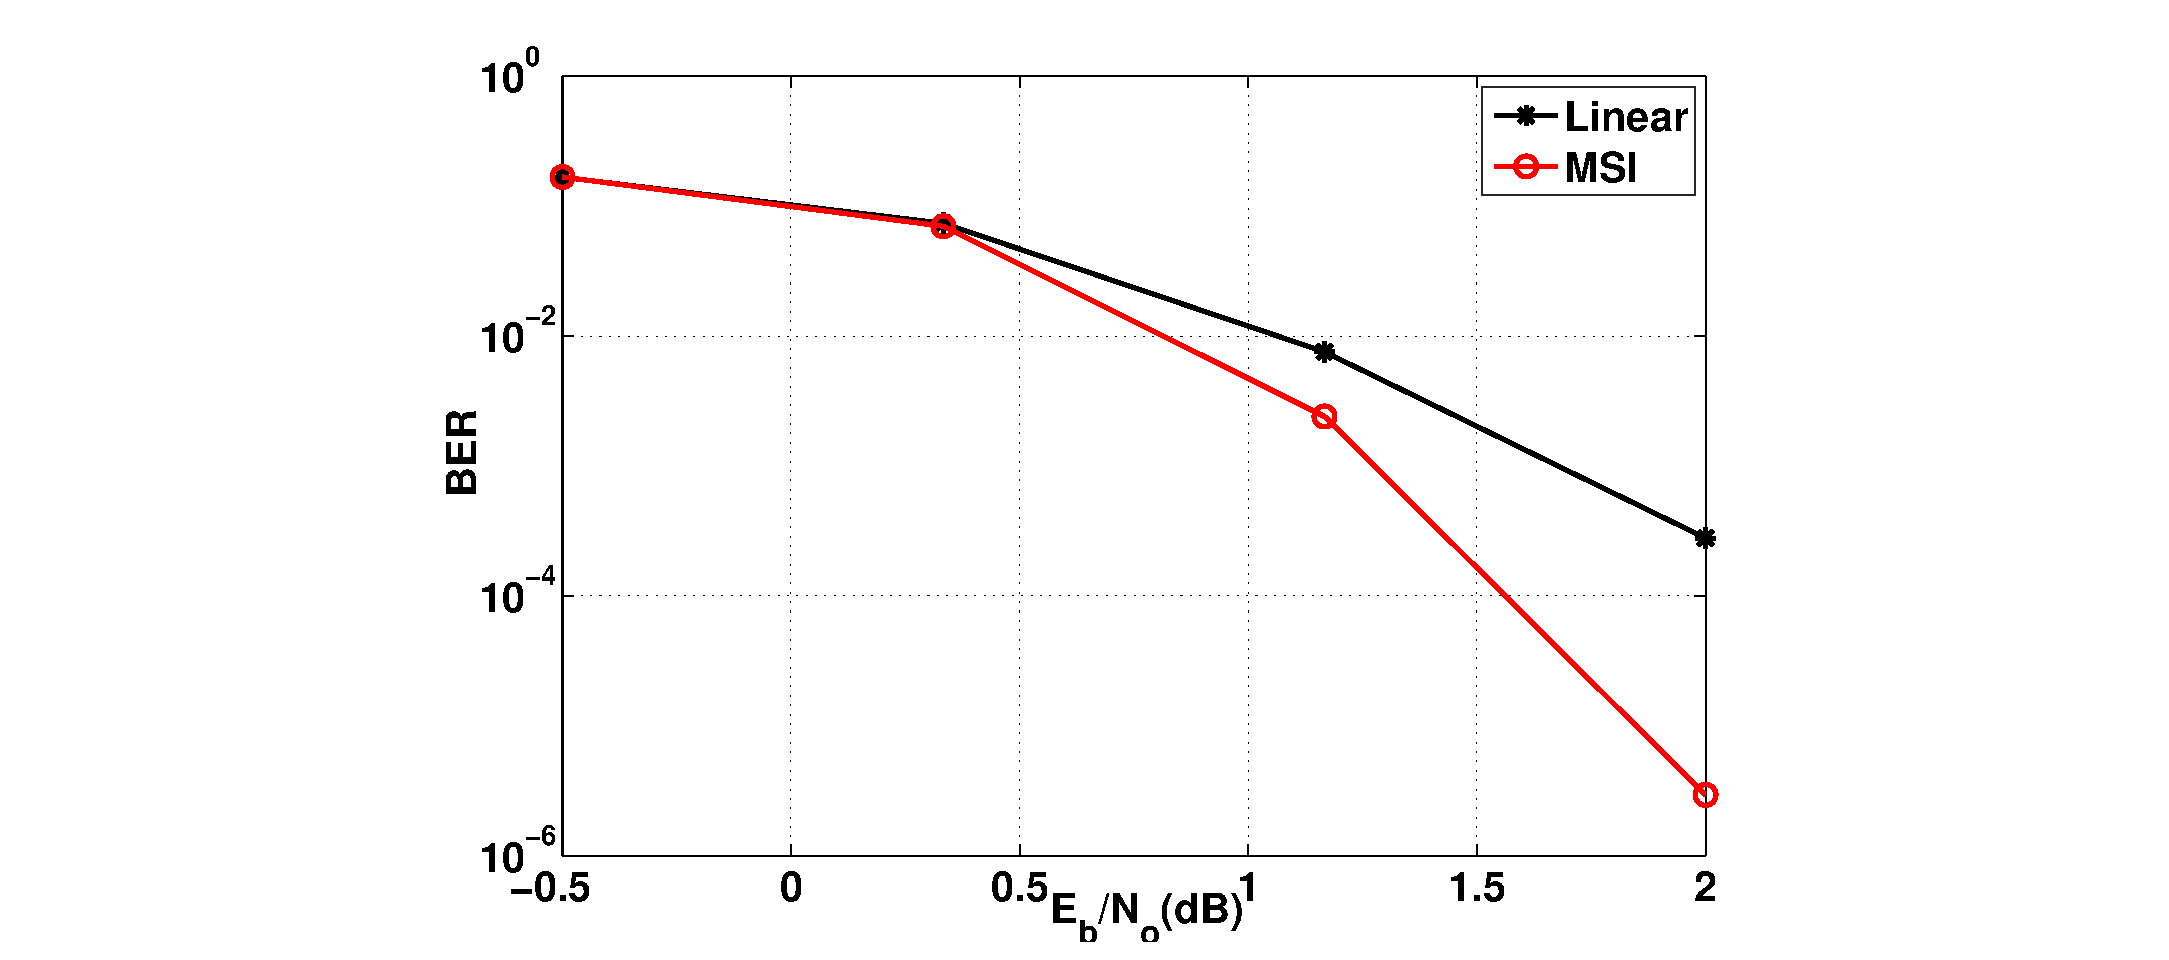
\includegraphics[width=1.35\paperwidth]{msi_linear_256_1000Frames_2.eps}
            };
        \end{tikzpicture}

\end{frame}

% slide 21
\begin{frame}
\frametitle{17. Results for $7/5$ Component Code. $N=1024$}
\begin{tikzpicture}[remember picture,overlay]
            \node[at=(current page.center)] {
                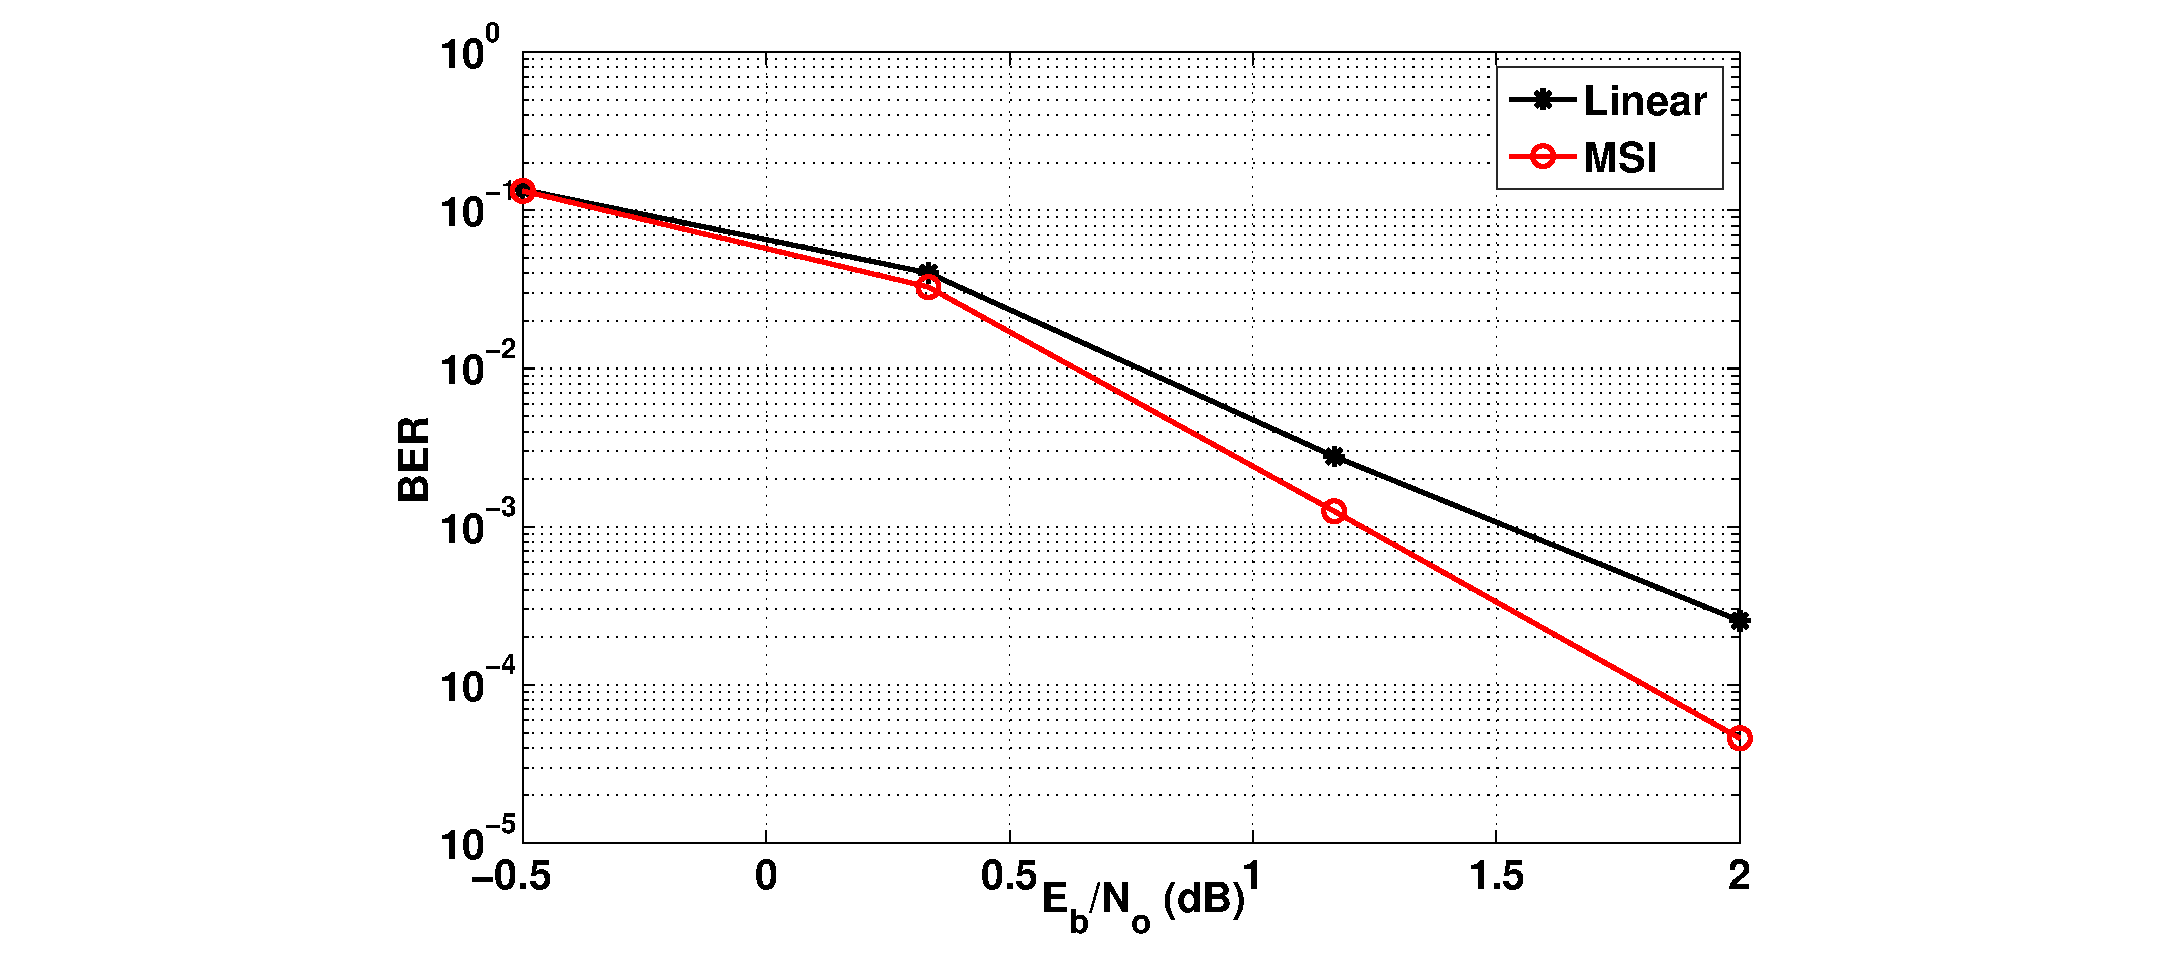
\includegraphics[width=1.35\paperwidth]{msi_linear_1024_1000_7_5Frames.eps}
            };
        \end{tikzpicture}

\end{frame}

% slide 19

\begin{frame}
\frametitle{17. Results for $5/7$ Component Code. $N=16384$}
 \begin{tikzpicture}[remember picture,overlay]
            \node[at=(current page.center)] {
                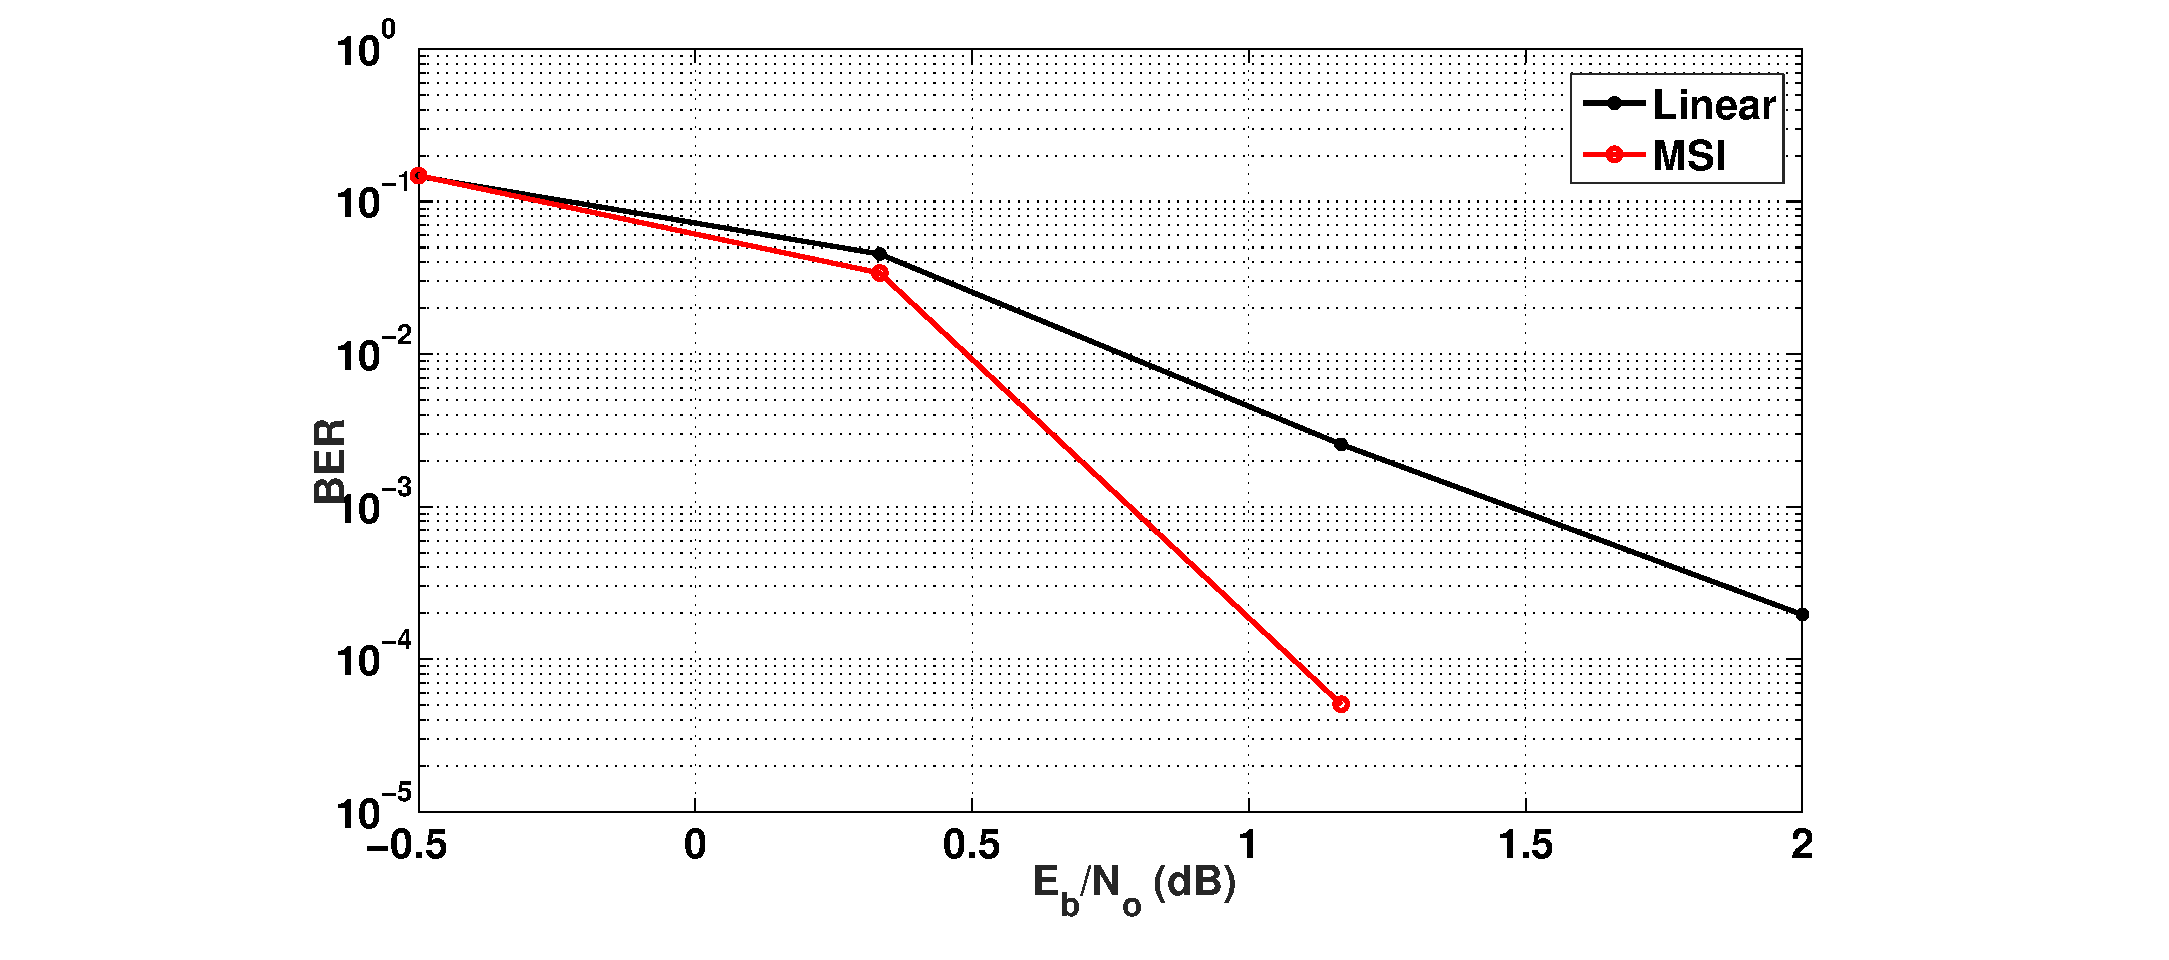
\includegraphics[width=1.35\paperwidth]{msi_linear_16384.eps}
            };
        \end{tikzpicture}

\end{frame}


% slide 19
\begin{frame}
\frametitle{18. Conclusion and Future Works}
\begin{block}{Conclusion}
\begin{itemize}
\setlength\itemsep{1em}
\item The multi-shift interleaver proposed.
\item Easier design than linear interleaver
\item Better performance than  linear interleaver for medium and long frame sizes. 
\end{itemize}
\end{block}

\begin{block}{Future Research }



\begin{itemize}
\setlength\itemsep{1em}
\item Deterministic interleaver that outperform random interleaver

\item Good interleaver design using BER bounds approach

\item LDPC code application







\end{itemize}
\end{block}
\end{frame}
\end{document}
